\documentclass[10pt]{article}
\usepackage[a4paper,left=11mm,right=11mm,top=18mm,bottom=11mm,
            includehead,headheight=14pt,headsep=4mm]{geometry}
\usepackage{amsmath}
\usepackage{microtype}
\usepackage{xcolor}
\usepackage{tikz}
\usepackage{fancyhdr}
\definecolor{ink}{HTML}{17212B}
\definecolor{muted}{HTML}{637083}
\definecolor{internalblue}{HTML}{245B78}
\definecolor{pendantgray}{HTML}{8795A5}
\definecolor{paperblue}{HTML}{EDF4F7}
\definecolor{specialseven}{HTML}{C4583C}
\tikzset{
  pendant edge/.style={draw=pendantgray,line width=0.8pt},
  internal edge/.style={draw=internalblue,line width=2.0pt},
  edge label/.style={font=\scriptsize,fill=white,fill opacity=.88,text opacity=1,
                     inner sep=1.1pt,sloped,above},
  internal vertex/.style={circle,fill=internalblue,draw=white,line width=.4pt,
                          minimum size=4.2pt,inner sep=0pt},
  leaf/.style={circle,fill=white,draw=ink,line width=.75pt,minimum size=5.2mm,
               inner sep=0pt,font=\small\bfseries,text=ink},
  special leaf/.style={leaf,fill=specialseven,draw=specialseven,text=white},
}
\pagestyle{fancy}
\fancyhf{}
\fancyhead[L]{\small\color{muted} Primitive integral Coxeter-balanced $G_2$ trees}
\fancyhead[R]{\small\color{muted}\thepage}
\renewcommand{\headrulewidth}{0pt}
\setlength{\parindent}{0pt}
\color{ink}
\begin{document}
\begin{center}
  {\Huge\bfseries Primitive integral $G_2$ trees}\par\vspace{3mm}
  {\large A symmetric atlas of the 51 rays of $\operatorname{Trop}(G_2/ P)$}\par\vspace{7mm}
  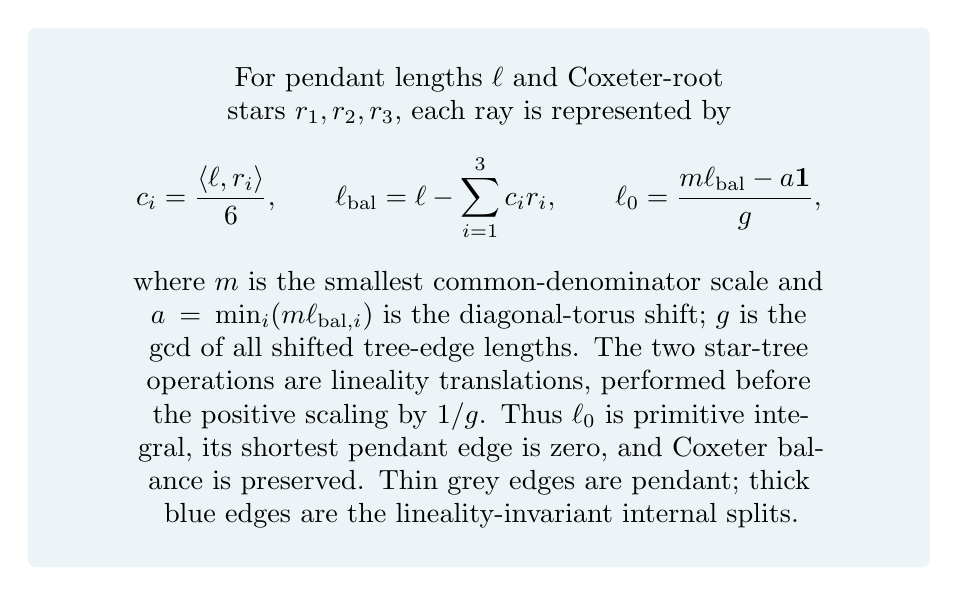
\begin{tikzpicture}
    \node[rounded corners=3pt,fill=paperblue,inner xsep=10mm,inner ysep=5mm,
          text width=.78\textwidth,align=center] {
      For pendant lengths $\ell$ and Coxeter-root stars $r_1,r_2,r_3$, each ray is
      represented by
      \[
        c_i=\frac{\langle\ell,r_i\rangle}{6},\qquad
        \ell_{\mathrm{bal}}=\ell-\sum_{i=1}^3c_i r_i,
        \qquad
        \ell_{0}=\frac{m\ell_{\mathrm{bal}}-a\mathbf 1}{g},
\]
      where $m$ is the smallest common-denominator scale and
      $a=\min_i(m\ell_{\mathrm{bal},i})$ is the diagonal-torus shift; $g$ is
      the gcd of all shifted tree-edge lengths. The two star-tree operations
      are lineality translations, performed before the positive scaling by
      $1/g$. Thus $\ell_0$ is primitive integral, its shortest pendant edge is
      zero, and Coxeter balance is preserved. Thin grey edges are pendant;
      thick blue edges are the lineality-invariant internal splits.
    };
  \end{tikzpicture}
\end{center}
\vfill
\begin{center}\color{muted}
Taxon $7$ is the rust-colored top vertex of every regular heptagon. Internal
vertices use a harmonic layout, zero-length internal refinements are contracted,
and every label is integral.
\end{center}
\clearpage

\begin{tikzpicture}
\node[rounded corners=2pt,fill=paperblue,inner xsep=5mm,inner ysep=2.2mm,text width=.94\textwidth] {\Large\bfseries Orbit 1\hfill\normalsize 12 rays};
\end{tikzpicture}\par\vspace{1mm}
{\small\color{muted} Ray indices: 1, 4, 23, 24, 38, 39, 42, 43, 48, 49, 50, 51}\par\vspace{2mm}
\begin{minipage}[t][0.285\textheight][t]{0.485\textwidth}
\centering
{\large\bfseries Ray 1}\par
{\scriptsize\color{muted} Coxeter shift $c=(\frac{7}{2},\,\frac{21}{2},\,-14)$}\par
{\scriptsize\color{muted} integral scale $m=2$, diagonal shift $a=-170$, gcd $g=105$}\par\vspace{1mm}
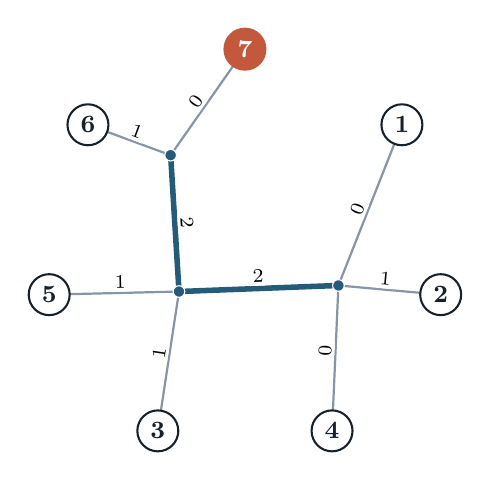
\begin{tikzpicture}[x=1cm,y=1cm]
\coordinate (v1) at (1.99367,1.58990);
\coordinate (v2) at (2.48607,-0.56743);
\coordinate (v3) at (-1.10640,-2.29747);
\coordinate (v4) at (1.10640,-2.29747);
\coordinate (v5) at (-2.48607,-0.56743);
\coordinate (v6) at (-1.99367,1.58990);
\coordinate (v7) at (0.00000,2.55000);
\coordinate (v8) at (-0.94363,1.20400);
\coordinate (v9) at (1.18723,-0.45073);
\coordinate (v10) at (-0.83722,-0.52791);
\draw[internal edge] (v8) -- node[edge label,pos=0.50] {$2$} (v10);
\draw[internal edge] (v9) -- node[edge label,pos=0.50] {$2$} (v10);
\draw[pendant edge] (v1) -- node[edge label,pos=0.55] {$0$} (v9);
\draw[pendant edge] (v2) -- node[edge label,pos=0.55] {$1$} (v9);
\draw[pendant edge] (v3) -- node[edge label,pos=0.55] {$1$} (v10);
\draw[pendant edge] (v4) -- node[edge label,pos=0.55] {$0$} (v9);
\draw[pendant edge] (v5) -- node[edge label,pos=0.55] {$1$} (v10);
\draw[pendant edge] (v6) -- node[edge label,pos=0.55] {$1$} (v8);
\draw[pendant edge] (v7) -- node[edge label,pos=0.55] {$0$} (v8);
\node[internal vertex] at (v8) {};
\node[internal vertex] at (v9) {};
\node[internal vertex] at (v10) {};
\node[leaf] at (v1) {1};
\node[leaf] at (v2) {2};
\node[leaf] at (v3) {3};
\node[leaf] at (v4) {4};
\node[leaf] at (v5) {5};
\node[leaf] at (v6) {6};
\node[special leaf] at (v7) {7};
\end{tikzpicture}
\end{minipage}
\hfill
\begin{minipage}[t][0.285\textheight][t]{0.485\textwidth}
\centering
{\large\bfseries Ray 4}\par
{\scriptsize\color{muted} Coxeter shift $c=(-\frac{7}{2},\,14,\,-\frac{21}{2})$}\par
{\scriptsize\color{muted} integral scale $m=2$, diagonal shift $a=-170$, gcd $g=105$}\par\vspace{1mm}
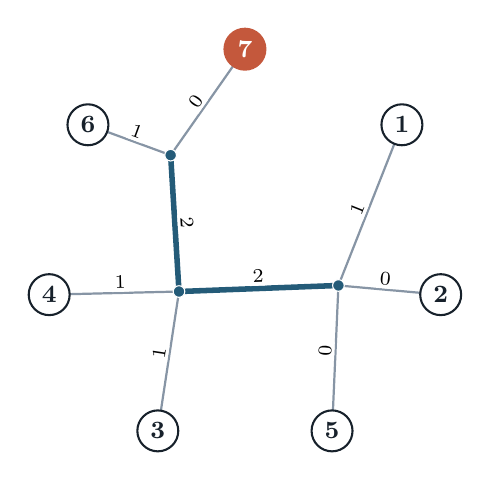
\begin{tikzpicture}[x=1cm,y=1cm]
\coordinate (v1) at (1.99367,1.58990);
\coordinate (v2) at (2.48607,-0.56743);
\coordinate (v3) at (-1.10640,-2.29747);
\coordinate (v4) at (-2.48607,-0.56743);
\coordinate (v5) at (1.10640,-2.29747);
\coordinate (v6) at (-1.99367,1.58990);
\coordinate (v7) at (0.00000,2.55000);
\coordinate (v8) at (-0.94363,1.20400);
\coordinate (v9) at (1.18723,-0.45073);
\coordinate (v10) at (-0.83722,-0.52791);
\draw[internal edge] (v8) -- node[edge label,pos=0.50] {$2$} (v10);
\draw[internal edge] (v9) -- node[edge label,pos=0.50] {$2$} (v10);
\draw[pendant edge] (v1) -- node[edge label,pos=0.55] {$1$} (v9);
\draw[pendant edge] (v2) -- node[edge label,pos=0.55] {$0$} (v9);
\draw[pendant edge] (v3) -- node[edge label,pos=0.55] {$1$} (v10);
\draw[pendant edge] (v4) -- node[edge label,pos=0.55] {$1$} (v10);
\draw[pendant edge] (v5) -- node[edge label,pos=0.55] {$0$} (v9);
\draw[pendant edge] (v6) -- node[edge label,pos=0.55] {$1$} (v8);
\draw[pendant edge] (v7) -- node[edge label,pos=0.55] {$0$} (v8);
\node[internal vertex] at (v8) {};
\node[internal vertex] at (v9) {};
\node[internal vertex] at (v10) {};
\node[leaf] at (v1) {1};
\node[leaf] at (v2) {2};
\node[leaf] at (v3) {3};
\node[leaf] at (v4) {4};
\node[leaf] at (v5) {5};
\node[leaf] at (v6) {6};
\node[special leaf] at (v7) {7};
\end{tikzpicture}
\end{minipage}
\par\vspace{1mm}
\begin{minipage}[t][0.285\textheight][t]{0.485\textwidth}
\centering
{\large\bfseries Ray 23}\par
{\scriptsize\color{muted} Coxeter shift $c=(-\frac{21}{2},\,-\frac{7}{2},\,14)$}\par
{\scriptsize\color{muted} integral scale $m=2$, diagonal shift $a=-170$, gcd $g=105$}\par\vspace{1mm}
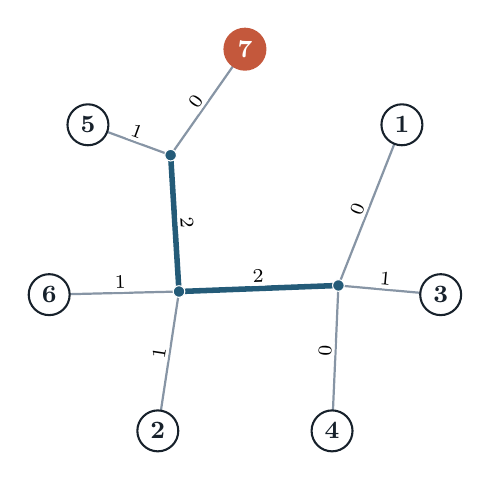
\begin{tikzpicture}[x=1cm,y=1cm]
\coordinate (v1) at (1.99367,1.58990);
\coordinate (v2) at (-1.10640,-2.29747);
\coordinate (v3) at (2.48607,-0.56743);
\coordinate (v4) at (1.10640,-2.29747);
\coordinate (v5) at (-1.99367,1.58990);
\coordinate (v6) at (-2.48607,-0.56743);
\coordinate (v7) at (0.00000,2.55000);
\coordinate (v8) at (-0.94363,1.20400);
\coordinate (v9) at (1.18723,-0.45073);
\coordinate (v10) at (-0.83722,-0.52791);
\draw[internal edge] (v8) -- node[edge label,pos=0.50] {$2$} (v10);
\draw[internal edge] (v9) -- node[edge label,pos=0.50] {$2$} (v10);
\draw[pendant edge] (v1) -- node[edge label,pos=0.55] {$0$} (v9);
\draw[pendant edge] (v2) -- node[edge label,pos=0.55] {$1$} (v10);
\draw[pendant edge] (v3) -- node[edge label,pos=0.55] {$1$} (v9);
\draw[pendant edge] (v4) -- node[edge label,pos=0.55] {$0$} (v9);
\draw[pendant edge] (v5) -- node[edge label,pos=0.55] {$1$} (v8);
\draw[pendant edge] (v6) -- node[edge label,pos=0.55] {$1$} (v10);
\draw[pendant edge] (v7) -- node[edge label,pos=0.55] {$0$} (v8);
\node[internal vertex] at (v8) {};
\node[internal vertex] at (v9) {};
\node[internal vertex] at (v10) {};
\node[leaf] at (v1) {1};
\node[leaf] at (v2) {2};
\node[leaf] at (v3) {3};
\node[leaf] at (v4) {4};
\node[leaf] at (v5) {5};
\node[leaf] at (v6) {6};
\node[special leaf] at (v7) {7};
\end{tikzpicture}
\end{minipage}
\hfill
\begin{minipage}[t][0.285\textheight][t]{0.485\textwidth}
\centering
{\large\bfseries Ray 24}\par
{\scriptsize\color{muted} Coxeter shift $c=(\frac{21}{2},\,-14,\,\frac{7}{2})$}\par
{\scriptsize\color{muted} integral scale $m=2$, diagonal shift $a=-170$, gcd $g=105$}\par\vspace{1mm}
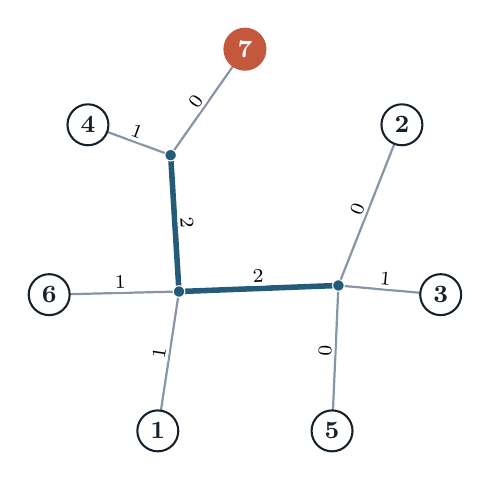
\begin{tikzpicture}[x=1cm,y=1cm]
\coordinate (v1) at (-1.10640,-2.29747);
\coordinate (v2) at (1.99367,1.58990);
\coordinate (v3) at (2.48607,-0.56743);
\coordinate (v4) at (-1.99367,1.58990);
\coordinate (v5) at (1.10640,-2.29747);
\coordinate (v6) at (-2.48607,-0.56743);
\coordinate (v7) at (0.00000,2.55000);
\coordinate (v8) at (-0.94363,1.20400);
\coordinate (v9) at (-0.83722,-0.52791);
\coordinate (v10) at (1.18723,-0.45073);
\draw[internal edge] (v8) -- node[edge label,pos=0.50] {$2$} (v9);
\draw[internal edge] (v9) -- node[edge label,pos=0.50] {$2$} (v10);
\draw[pendant edge] (v1) -- node[edge label,pos=0.55] {$1$} (v9);
\draw[pendant edge] (v2) -- node[edge label,pos=0.55] {$0$} (v10);
\draw[pendant edge] (v3) -- node[edge label,pos=0.55] {$1$} (v10);
\draw[pendant edge] (v4) -- node[edge label,pos=0.55] {$1$} (v8);
\draw[pendant edge] (v5) -- node[edge label,pos=0.55] {$0$} (v10);
\draw[pendant edge] (v6) -- node[edge label,pos=0.55] {$1$} (v9);
\draw[pendant edge] (v7) -- node[edge label,pos=0.55] {$0$} (v8);
\node[internal vertex] at (v8) {};
\node[internal vertex] at (v9) {};
\node[internal vertex] at (v10) {};
\node[leaf] at (v1) {1};
\node[leaf] at (v2) {2};
\node[leaf] at (v3) {3};
\node[leaf] at (v4) {4};
\node[leaf] at (v5) {5};
\node[leaf] at (v6) {6};
\node[special leaf] at (v7) {7};
\end{tikzpicture}
\end{minipage}
\par\vspace{1mm}
\begin{minipage}[t][0.285\textheight][t]{0.485\textwidth}
\centering
{\large\bfseries Ray 38}\par
{\scriptsize\color{muted} Coxeter shift $c=(14,\,-\frac{7}{2},\,-\frac{21}{2})$}\par
{\scriptsize\color{muted} integral scale $m=2$, diagonal shift $a=-170$, gcd $g=105$}\par\vspace{1mm}
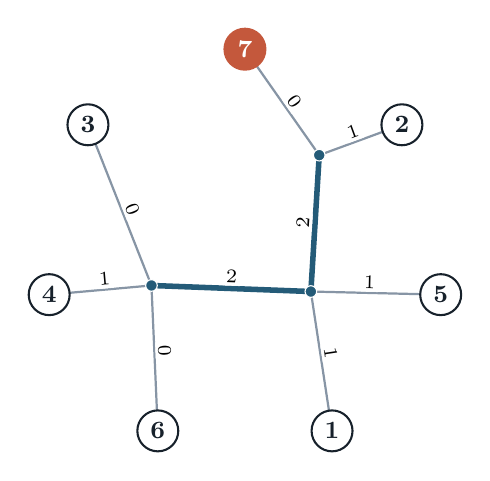
\begin{tikzpicture}[x=1cm,y=1cm]
\coordinate (v1) at (1.10640,-2.29747);
\coordinate (v2) at (1.99367,1.58990);
\coordinate (v3) at (-1.99367,1.58990);
\coordinate (v4) at (-2.48607,-0.56743);
\coordinate (v5) at (2.48607,-0.56743);
\coordinate (v6) at (-1.10640,-2.29747);
\coordinate (v7) at (0.00000,2.55000);
\coordinate (v8) at (0.94363,1.20400);
\coordinate (v9) at (0.83722,-0.52791);
\coordinate (v10) at (-1.18723,-0.45073);
\draw[internal edge] (v8) -- node[edge label,pos=0.50] {$2$} (v9);
\draw[internal edge] (v9) -- node[edge label,pos=0.50] {$2$} (v10);
\draw[pendant edge] (v1) -- node[edge label,pos=0.55] {$1$} (v9);
\draw[pendant edge] (v2) -- node[edge label,pos=0.55] {$1$} (v8);
\draw[pendant edge] (v3) -- node[edge label,pos=0.55] {$0$} (v10);
\draw[pendant edge] (v4) -- node[edge label,pos=0.55] {$1$} (v10);
\draw[pendant edge] (v5) -- node[edge label,pos=0.55] {$1$} (v9);
\draw[pendant edge] (v6) -- node[edge label,pos=0.55] {$0$} (v10);
\draw[pendant edge] (v7) -- node[edge label,pos=0.55] {$0$} (v8);
\node[internal vertex] at (v8) {};
\node[internal vertex] at (v9) {};
\node[internal vertex] at (v10) {};
\node[leaf] at (v1) {1};
\node[leaf] at (v2) {2};
\node[leaf] at (v3) {3};
\node[leaf] at (v4) {4};
\node[leaf] at (v5) {5};
\node[leaf] at (v6) {6};
\node[special leaf] at (v7) {7};
\end{tikzpicture}
\end{minipage}
\hfill
\begin{minipage}[t][0.285\textheight][t]{0.485\textwidth}
\centering
{\large\bfseries Ray 39}\par
{\scriptsize\color{muted} Coxeter shift $c=(-14,\,\frac{21}{2},\,\frac{7}{2})$}\par
{\scriptsize\color{muted} integral scale $m=2$, diagonal shift $a=-170$, gcd $g=105$}\par\vspace{1mm}
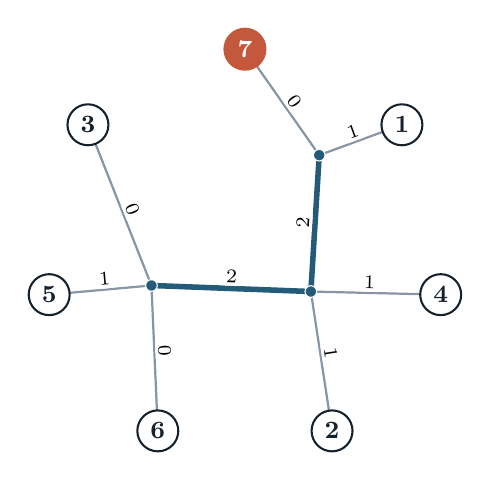
\begin{tikzpicture}[x=1cm,y=1cm]
\coordinate (v1) at (1.99367,1.58990);
\coordinate (v2) at (1.10640,-2.29747);
\coordinate (v3) at (-1.99367,1.58990);
\coordinate (v4) at (2.48607,-0.56743);
\coordinate (v5) at (-2.48607,-0.56743);
\coordinate (v6) at (-1.10640,-2.29747);
\coordinate (v7) at (0.00000,2.55000);
\coordinate (v8) at (0.94363,1.20400);
\coordinate (v9) at (0.83722,-0.52791);
\coordinate (v10) at (-1.18723,-0.45073);
\draw[internal edge] (v8) -- node[edge label,pos=0.50] {$2$} (v9);
\draw[internal edge] (v9) -- node[edge label,pos=0.50] {$2$} (v10);
\draw[pendant edge] (v1) -- node[edge label,pos=0.55] {$1$} (v8);
\draw[pendant edge] (v2) -- node[edge label,pos=0.55] {$1$} (v9);
\draw[pendant edge] (v3) -- node[edge label,pos=0.55] {$0$} (v10);
\draw[pendant edge] (v4) -- node[edge label,pos=0.55] {$1$} (v9);
\draw[pendant edge] (v5) -- node[edge label,pos=0.55] {$1$} (v10);
\draw[pendant edge] (v6) -- node[edge label,pos=0.55] {$0$} (v10);
\draw[pendant edge] (v7) -- node[edge label,pos=0.55] {$0$} (v8);
\node[internal vertex] at (v8) {};
\node[internal vertex] at (v9) {};
\node[internal vertex] at (v10) {};
\node[leaf] at (v1) {1};
\node[leaf] at (v2) {2};
\node[leaf] at (v3) {3};
\node[leaf] at (v4) {4};
\node[leaf] at (v5) {5};
\node[leaf] at (v6) {6};
\node[special leaf] at (v7) {7};
\end{tikzpicture}
\end{minipage}
\par\vspace{1mm}
\clearpage

\begin{tikzpicture}
\node[rounded corners=2pt,fill=paperblue,inner xsep=5mm,inner ysep=2.2mm,text width=.94\textwidth] {\Large\bfseries Orbit 1 (continued)\hfill\normalsize 12 rays};
\end{tikzpicture}\par\vspace{1mm}
{\small\color{muted} Ray indices: 1, 4, 23, 24, 38, 39, 42, 43, 48, 49, 50, 51}\par\vspace{2mm}
\begin{minipage}[t][0.285\textheight][t]{0.485\textwidth}
\centering
{\large\bfseries Ray 42}\par
{\scriptsize\color{muted} Coxeter shift $c=(\frac{7}{2},\,-14,\,\frac{21}{2})$}\par
{\scriptsize\color{muted} integral scale $m=2$, diagonal shift $a=-170$, gcd $g=105$}\par\vspace{1mm}
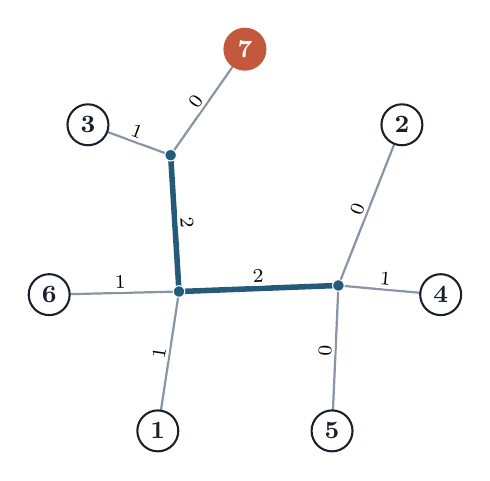
\begin{tikzpicture}[x=1cm,y=1cm]
\coordinate (v1) at (-1.10640,-2.29747);
\coordinate (v2) at (1.99367,1.58990);
\coordinate (v3) at (-1.99367,1.58990);
\coordinate (v4) at (2.48607,-0.56743);
\coordinate (v5) at (1.10640,-2.29747);
\coordinate (v6) at (-2.48607,-0.56743);
\coordinate (v7) at (0.00000,2.55000);
\coordinate (v8) at (-0.94363,1.20400);
\coordinate (v9) at (-0.83722,-0.52791);
\coordinate (v10) at (1.18723,-0.45073);
\draw[internal edge] (v8) -- node[edge label,pos=0.50] {$2$} (v9);
\draw[internal edge] (v9) -- node[edge label,pos=0.50] {$2$} (v10);
\draw[pendant edge] (v1) -- node[edge label,pos=0.55] {$1$} (v9);
\draw[pendant edge] (v2) -- node[edge label,pos=0.55] {$0$} (v10);
\draw[pendant edge] (v3) -- node[edge label,pos=0.55] {$1$} (v8);
\draw[pendant edge] (v4) -- node[edge label,pos=0.55] {$1$} (v10);
\draw[pendant edge] (v5) -- node[edge label,pos=0.55] {$0$} (v10);
\draw[pendant edge] (v6) -- node[edge label,pos=0.55] {$1$} (v9);
\draw[pendant edge] (v7) -- node[edge label,pos=0.55] {$0$} (v8);
\node[internal vertex] at (v8) {};
\node[internal vertex] at (v9) {};
\node[internal vertex] at (v10) {};
\node[leaf] at (v1) {1};
\node[leaf] at (v2) {2};
\node[leaf] at (v3) {3};
\node[leaf] at (v4) {4};
\node[leaf] at (v5) {5};
\node[leaf] at (v6) {6};
\node[special leaf] at (v7) {7};
\end{tikzpicture}
\end{minipage}
\hfill
\begin{minipage}[t][0.285\textheight][t]{0.485\textwidth}
\centering
{\large\bfseries Ray 43}\par
{\scriptsize\color{muted} Coxeter shift $c=(-\frac{7}{2},\,-\frac{21}{2},\,14)$}\par
{\scriptsize\color{muted} integral scale $m=2$, diagonal shift $a=-170$, gcd $g=105$}\par\vspace{1mm}
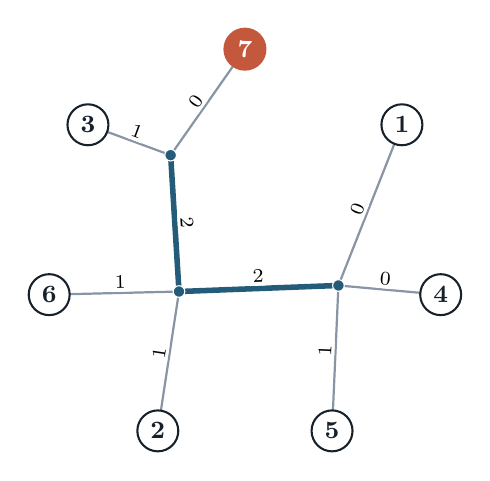
\begin{tikzpicture}[x=1cm,y=1cm]
\coordinate (v1) at (1.99367,1.58990);
\coordinate (v2) at (-1.10640,-2.29747);
\coordinate (v3) at (-1.99367,1.58990);
\coordinate (v4) at (2.48607,-0.56743);
\coordinate (v5) at (1.10640,-2.29747);
\coordinate (v6) at (-2.48607,-0.56743);
\coordinate (v7) at (0.00000,2.55000);
\coordinate (v8) at (-0.94363,1.20400);
\coordinate (v9) at (1.18723,-0.45073);
\coordinate (v10) at (-0.83722,-0.52791);
\draw[internal edge] (v8) -- node[edge label,pos=0.50] {$2$} (v10);
\draw[internal edge] (v9) -- node[edge label,pos=0.50] {$2$} (v10);
\draw[pendant edge] (v1) -- node[edge label,pos=0.55] {$0$} (v9);
\draw[pendant edge] (v2) -- node[edge label,pos=0.55] {$1$} (v10);
\draw[pendant edge] (v3) -- node[edge label,pos=0.55] {$1$} (v8);
\draw[pendant edge] (v4) -- node[edge label,pos=0.55] {$0$} (v9);
\draw[pendant edge] (v5) -- node[edge label,pos=0.55] {$1$} (v9);
\draw[pendant edge] (v6) -- node[edge label,pos=0.55] {$1$} (v10);
\draw[pendant edge] (v7) -- node[edge label,pos=0.55] {$0$} (v8);
\node[internal vertex] at (v8) {};
\node[internal vertex] at (v9) {};
\node[internal vertex] at (v10) {};
\node[leaf] at (v1) {1};
\node[leaf] at (v2) {2};
\node[leaf] at (v3) {3};
\node[leaf] at (v4) {4};
\node[leaf] at (v5) {5};
\node[leaf] at (v6) {6};
\node[special leaf] at (v7) {7};
\end{tikzpicture}
\end{minipage}
\par\vspace{1mm}
\begin{minipage}[t][0.285\textheight][t]{0.485\textwidth}
\centering
{\large\bfseries Ray 48}\par
{\scriptsize\color{muted} Coxeter shift $c=(-14,\,\frac{7}{2},\,\frac{21}{2})$}\par
{\scriptsize\color{muted} integral scale $m=2$, diagonal shift $a=-170$, gcd $g=105$}\par\vspace{1mm}
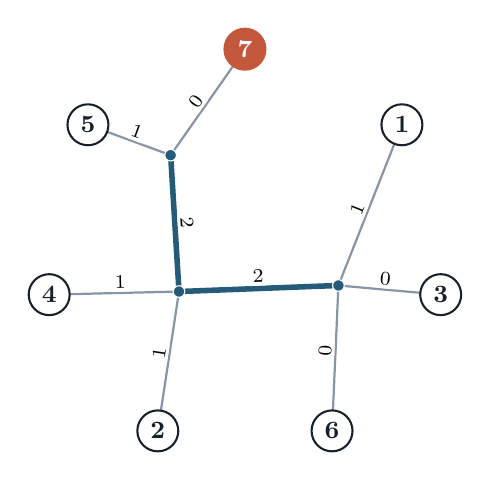
\begin{tikzpicture}[x=1cm,y=1cm]
\coordinate (v1) at (1.99367,1.58990);
\coordinate (v2) at (-1.10640,-2.29747);
\coordinate (v3) at (2.48607,-0.56743);
\coordinate (v4) at (-2.48607,-0.56743);
\coordinate (v5) at (-1.99367,1.58990);
\coordinate (v6) at (1.10640,-2.29747);
\coordinate (v7) at (0.00000,2.55000);
\coordinate (v8) at (-0.94363,1.20400);
\coordinate (v9) at (1.18723,-0.45073);
\coordinate (v10) at (-0.83722,-0.52791);
\draw[internal edge] (v8) -- node[edge label,pos=0.50] {$2$} (v10);
\draw[internal edge] (v9) -- node[edge label,pos=0.50] {$2$} (v10);
\draw[pendant edge] (v1) -- node[edge label,pos=0.55] {$1$} (v9);
\draw[pendant edge] (v2) -- node[edge label,pos=0.55] {$1$} (v10);
\draw[pendant edge] (v3) -- node[edge label,pos=0.55] {$0$} (v9);
\draw[pendant edge] (v4) -- node[edge label,pos=0.55] {$1$} (v10);
\draw[pendant edge] (v5) -- node[edge label,pos=0.55] {$1$} (v8);
\draw[pendant edge] (v6) -- node[edge label,pos=0.55] {$0$} (v9);
\draw[pendant edge] (v7) -- node[edge label,pos=0.55] {$0$} (v8);
\node[internal vertex] at (v8) {};
\node[internal vertex] at (v9) {};
\node[internal vertex] at (v10) {};
\node[leaf] at (v1) {1};
\node[leaf] at (v2) {2};
\node[leaf] at (v3) {3};
\node[leaf] at (v4) {4};
\node[leaf] at (v5) {5};
\node[leaf] at (v6) {6};
\node[special leaf] at (v7) {7};
\end{tikzpicture}
\end{minipage}
\hfill
\begin{minipage}[t][0.285\textheight][t]{0.485\textwidth}
\centering
{\large\bfseries Ray 49}\par
{\scriptsize\color{muted} Coxeter shift $c=(14,\,-\frac{21}{2},\,-\frac{7}{2})$}\par
{\scriptsize\color{muted} integral scale $m=2$, diagonal shift $a=-170$, gcd $g=105$}\par\vspace{1mm}
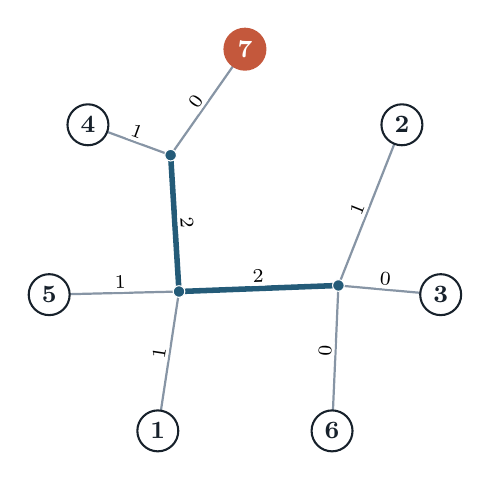
\begin{tikzpicture}[x=1cm,y=1cm]
\coordinate (v1) at (-1.10640,-2.29747);
\coordinate (v2) at (1.99367,1.58990);
\coordinate (v3) at (2.48607,-0.56743);
\coordinate (v4) at (-1.99367,1.58990);
\coordinate (v5) at (-2.48607,-0.56743);
\coordinate (v6) at (1.10640,-2.29747);
\coordinate (v7) at (0.00000,2.55000);
\coordinate (v8) at (-0.94363,1.20400);
\coordinate (v9) at (-0.83722,-0.52791);
\coordinate (v10) at (1.18723,-0.45073);
\draw[internal edge] (v8) -- node[edge label,pos=0.50] {$2$} (v9);
\draw[internal edge] (v9) -- node[edge label,pos=0.50] {$2$} (v10);
\draw[pendant edge] (v1) -- node[edge label,pos=0.55] {$1$} (v9);
\draw[pendant edge] (v2) -- node[edge label,pos=0.55] {$1$} (v10);
\draw[pendant edge] (v3) -- node[edge label,pos=0.55] {$0$} (v10);
\draw[pendant edge] (v4) -- node[edge label,pos=0.55] {$1$} (v8);
\draw[pendant edge] (v5) -- node[edge label,pos=0.55] {$1$} (v9);
\draw[pendant edge] (v6) -- node[edge label,pos=0.55] {$0$} (v10);
\draw[pendant edge] (v7) -- node[edge label,pos=0.55] {$0$} (v8);
\node[internal vertex] at (v8) {};
\node[internal vertex] at (v9) {};
\node[internal vertex] at (v10) {};
\node[leaf] at (v1) {1};
\node[leaf] at (v2) {2};
\node[leaf] at (v3) {3};
\node[leaf] at (v4) {4};
\node[leaf] at (v5) {5};
\node[leaf] at (v6) {6};
\node[special leaf] at (v7) {7};
\end{tikzpicture}
\end{minipage}
\par\vspace{1mm}
\begin{minipage}[t][0.285\textheight][t]{0.485\textwidth}
\centering
{\large\bfseries Ray 50}\par
{\scriptsize\color{muted} Coxeter shift $c=(\frac{21}{2},\,\frac{7}{2},\,-14)$}\par
{\scriptsize\color{muted} integral scale $m=2$, diagonal shift $a=-170$, gcd $g=105$}\par\vspace{1mm}
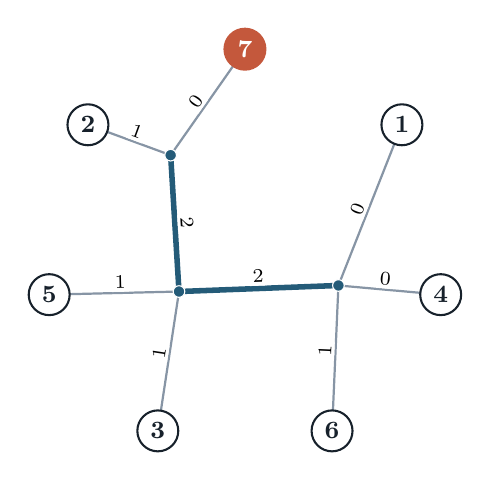
\begin{tikzpicture}[x=1cm,y=1cm]
\coordinate (v1) at (1.99367,1.58990);
\coordinate (v2) at (-1.99367,1.58990);
\coordinate (v3) at (-1.10640,-2.29747);
\coordinate (v4) at (2.48607,-0.56743);
\coordinate (v5) at (-2.48607,-0.56743);
\coordinate (v6) at (1.10640,-2.29747);
\coordinate (v7) at (0.00000,2.55000);
\coordinate (v8) at (-0.94363,1.20400);
\coordinate (v9) at (1.18723,-0.45073);
\coordinate (v10) at (-0.83722,-0.52791);
\draw[internal edge] (v8) -- node[edge label,pos=0.50] {$2$} (v10);
\draw[internal edge] (v9) -- node[edge label,pos=0.50] {$2$} (v10);
\draw[pendant edge] (v1) -- node[edge label,pos=0.55] {$0$} (v9);
\draw[pendant edge] (v2) -- node[edge label,pos=0.55] {$1$} (v8);
\draw[pendant edge] (v3) -- node[edge label,pos=0.55] {$1$} (v10);
\draw[pendant edge] (v4) -- node[edge label,pos=0.55] {$0$} (v9);
\draw[pendant edge] (v5) -- node[edge label,pos=0.55] {$1$} (v10);
\draw[pendant edge] (v6) -- node[edge label,pos=0.55] {$1$} (v9);
\draw[pendant edge] (v7) -- node[edge label,pos=0.55] {$0$} (v8);
\node[internal vertex] at (v8) {};
\node[internal vertex] at (v9) {};
\node[internal vertex] at (v10) {};
\node[leaf] at (v1) {1};
\node[leaf] at (v2) {2};
\node[leaf] at (v3) {3};
\node[leaf] at (v4) {4};
\node[leaf] at (v5) {5};
\node[leaf] at (v6) {6};
\node[special leaf] at (v7) {7};
\end{tikzpicture}
\end{minipage}
\hfill
\begin{minipage}[t][0.285\textheight][t]{0.485\textwidth}
\centering
{\large\bfseries Ray 51}\par
{\scriptsize\color{muted} Coxeter shift $c=(-\frac{21}{2},\,14,\,-\frac{7}{2})$}\par
{\scriptsize\color{muted} integral scale $m=2$, diagonal shift $a=-170$, gcd $g=105$}\par\vspace{1mm}
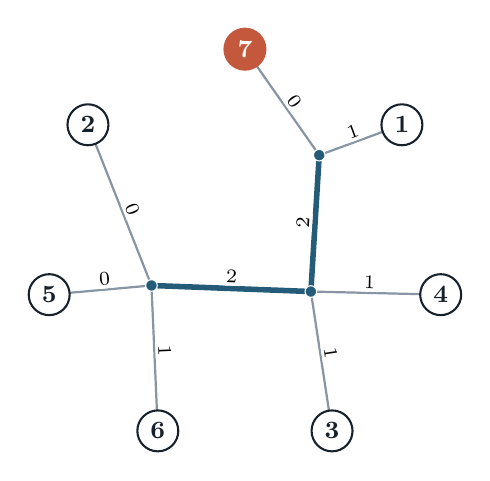
\begin{tikzpicture}[x=1cm,y=1cm]
\coordinate (v1) at (1.99367,1.58990);
\coordinate (v2) at (-1.99367,1.58990);
\coordinate (v3) at (1.10640,-2.29747);
\coordinate (v4) at (2.48607,-0.56743);
\coordinate (v5) at (-2.48607,-0.56743);
\coordinate (v6) at (-1.10640,-2.29747);
\coordinate (v7) at (0.00000,2.55000);
\coordinate (v8) at (0.94363,1.20400);
\coordinate (v9) at (-1.18723,-0.45073);
\coordinate (v10) at (0.83722,-0.52791);
\draw[internal edge] (v8) -- node[edge label,pos=0.50] {$2$} (v10);
\draw[internal edge] (v9) -- node[edge label,pos=0.50] {$2$} (v10);
\draw[pendant edge] (v1) -- node[edge label,pos=0.55] {$1$} (v8);
\draw[pendant edge] (v2) -- node[edge label,pos=0.55] {$0$} (v9);
\draw[pendant edge] (v3) -- node[edge label,pos=0.55] {$1$} (v10);
\draw[pendant edge] (v4) -- node[edge label,pos=0.55] {$1$} (v10);
\draw[pendant edge] (v5) -- node[edge label,pos=0.55] {$0$} (v9);
\draw[pendant edge] (v6) -- node[edge label,pos=0.55] {$1$} (v9);
\draw[pendant edge] (v7) -- node[edge label,pos=0.55] {$0$} (v8);
\node[internal vertex] at (v8) {};
\node[internal vertex] at (v9) {};
\node[internal vertex] at (v10) {};
\node[leaf] at (v1) {1};
\node[leaf] at (v2) {2};
\node[leaf] at (v3) {3};
\node[leaf] at (v4) {4};
\node[leaf] at (v5) {5};
\node[leaf] at (v6) {6};
\node[special leaf] at (v7) {7};
\end{tikzpicture}
\end{minipage}
\par\vspace{1mm}
\clearpage

\begin{tikzpicture}
\node[rounded corners=2pt,fill=paperblue,inner xsep=5mm,inner ysep=2.2mm,text width=.94\textwidth] {\Large\bfseries Orbit 2\hfill\normalsize 12 rays};
\end{tikzpicture}\par\vspace{1mm}
{\small\color{muted} Ray indices: 2, 3, 5, 16, 25, 26, 27, 28, 31, 32, 46, 47}\par\vspace{2mm}
\begin{minipage}[t][0.285\textheight][t]{0.485\textwidth}
\centering
{\large\bfseries Ray 2}\par
{\scriptsize\color{muted} Coxeter shift $c=(0,\,\frac{21}{2},\,-\frac{21}{2})$}\par
{\scriptsize\color{muted} integral scale $m=2$, diagonal shift $a=-95$, gcd $g=35$}\par\vspace{1mm}
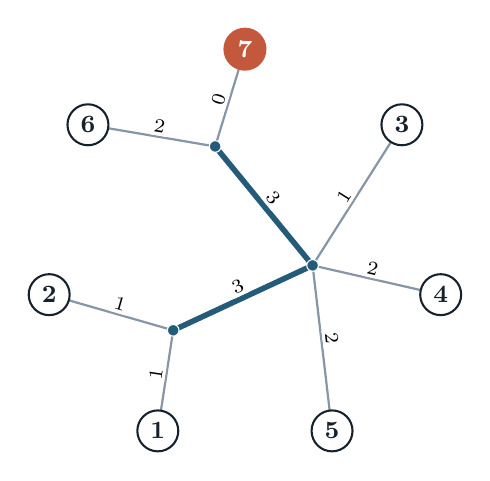
\begin{tikzpicture}[x=1cm,y=1cm]
\coordinate (v1) at (-1.10640,-2.29747);
\coordinate (v2) at (-2.48607,-0.56743);
\coordinate (v3) at (1.99367,1.58990);
\coordinate (v4) at (2.48607,-0.56743);
\coordinate (v5) at (1.10640,-2.29747);
\coordinate (v6) at (-1.99367,1.58990);
\coordinate (v7) at (0.00000,2.55000);
\coordinate (v8) at (-0.91102,-1.02035);
\coordinate (v9) at (-0.37809,1.31458);
\coordinate (v10) at (0.85941,-0.19615);
\draw[internal edge] (v8) -- node[edge label,pos=0.50] {$3$} (v10);
\draw[internal edge] (v9) -- node[edge label,pos=0.50] {$3$} (v10);
\draw[pendant edge] (v1) -- node[edge label,pos=0.55] {$1$} (v8);
\draw[pendant edge] (v2) -- node[edge label,pos=0.55] {$1$} (v8);
\draw[pendant edge] (v3) -- node[edge label,pos=0.55] {$1$} (v10);
\draw[pendant edge] (v4) -- node[edge label,pos=0.55] {$2$} (v10);
\draw[pendant edge] (v5) -- node[edge label,pos=0.55] {$2$} (v10);
\draw[pendant edge] (v6) -- node[edge label,pos=0.55] {$2$} (v9);
\draw[pendant edge] (v7) -- node[edge label,pos=0.55] {$0$} (v9);
\node[internal vertex] at (v8) {};
\node[internal vertex] at (v9) {};
\node[internal vertex] at (v10) {};
\node[leaf] at (v1) {1};
\node[leaf] at (v2) {2};
\node[leaf] at (v3) {3};
\node[leaf] at (v4) {4};
\node[leaf] at (v5) {5};
\node[leaf] at (v6) {6};
\node[special leaf] at (v7) {7};
\end{tikzpicture}
\end{minipage}
\hfill
\begin{minipage}[t][0.285\textheight][t]{0.485\textwidth}
\centering
{\large\bfseries Ray 3}\par
{\scriptsize\color{muted} Coxeter shift $c=(-\frac{7}{2},\,\frac{7}{2},\,0)$}\par
{\scriptsize\color{muted} integral scale $m=2$, diagonal shift $a=-120$, gcd $g=105$}\par\vspace{1mm}
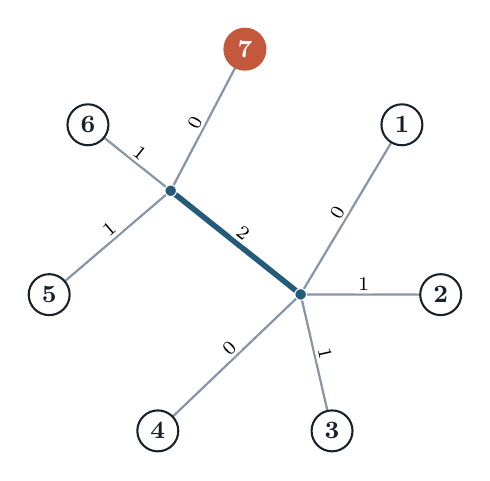
\begin{tikzpicture}[x=1cm,y=1cm]
\coordinate (v1) at (1.99367,1.58990);
\coordinate (v2) at (2.48607,-0.56743);
\coordinate (v3) at (1.10640,-2.29747);
\coordinate (v4) at (-1.10640,-2.29747);
\coordinate (v5) at (-2.48607,-0.56743);
\coordinate (v6) at (-1.99367,1.58990);
\coordinate (v7) at (0.00000,2.55000);
\coordinate (v8) at (-0.94310,0.75210);
\coordinate (v9) at (0.70733,-0.56407);
\draw[internal edge] (v8) -- node[edge label,pos=0.50] {$2$} (v9);
\draw[pendant edge] (v1) -- node[edge label,pos=0.55] {$0$} (v9);
\draw[pendant edge] (v2) -- node[edge label,pos=0.55] {$1$} (v9);
\draw[pendant edge] (v3) -- node[edge label,pos=0.55] {$1$} (v9);
\draw[pendant edge] (v4) -- node[edge label,pos=0.55] {$0$} (v9);
\draw[pendant edge] (v5) -- node[edge label,pos=0.55] {$1$} (v8);
\draw[pendant edge] (v6) -- node[edge label,pos=0.55] {$1$} (v8);
\draw[pendant edge] (v7) -- node[edge label,pos=0.55] {$0$} (v8);
\node[internal vertex] at (v8) {};
\node[internal vertex] at (v9) {};
\node[leaf] at (v1) {1};
\node[leaf] at (v2) {2};
\node[leaf] at (v3) {3};
\node[leaf] at (v4) {4};
\node[leaf] at (v5) {5};
\node[leaf] at (v6) {6};
\node[special leaf] at (v7) {7};
\end{tikzpicture}
\end{minipage}
\par\vspace{1mm}
\begin{minipage}[t][0.285\textheight][t]{0.485\textwidth}
\centering
{\large\bfseries Ray 5}\par
{\scriptsize\color{muted} Coxeter shift $c=(\frac{7}{2},\,0,\,-\frac{7}{2})$}\par
{\scriptsize\color{muted} integral scale $m=2$, diagonal shift $a=-120$, gcd $g=105$}\par\vspace{1mm}
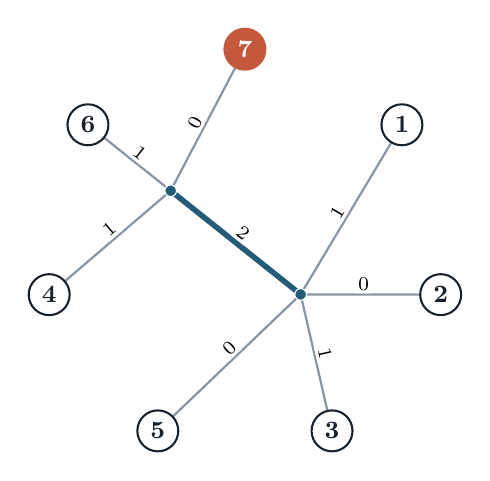
\begin{tikzpicture}[x=1cm,y=1cm]
\coordinate (v1) at (1.99367,1.58990);
\coordinate (v2) at (2.48607,-0.56743);
\coordinate (v3) at (1.10640,-2.29747);
\coordinate (v4) at (-2.48607,-0.56743);
\coordinate (v5) at (-1.10640,-2.29747);
\coordinate (v6) at (-1.99367,1.58990);
\coordinate (v7) at (0.00000,2.55000);
\coordinate (v8) at (-0.94310,0.75210);
\coordinate (v9) at (0.70733,-0.56407);
\draw[internal edge] (v8) -- node[edge label,pos=0.50] {$2$} (v9);
\draw[pendant edge] (v1) -- node[edge label,pos=0.55] {$1$} (v9);
\draw[pendant edge] (v2) -- node[edge label,pos=0.55] {$0$} (v9);
\draw[pendant edge] (v3) -- node[edge label,pos=0.55] {$1$} (v9);
\draw[pendant edge] (v4) -- node[edge label,pos=0.55] {$1$} (v8);
\draw[pendant edge] (v5) -- node[edge label,pos=0.55] {$0$} (v9);
\draw[pendant edge] (v6) -- node[edge label,pos=0.55] {$1$} (v8);
\draw[pendant edge] (v7) -- node[edge label,pos=0.55] {$0$} (v8);
\node[internal vertex] at (v8) {};
\node[internal vertex] at (v9) {};
\node[leaf] at (v1) {1};
\node[leaf] at (v2) {2};
\node[leaf] at (v3) {3};
\node[leaf] at (v4) {4};
\node[leaf] at (v5) {5};
\node[leaf] at (v6) {6};
\node[special leaf] at (v7) {7};
\end{tikzpicture}
\end{minipage}
\hfill
\begin{minipage}[t][0.285\textheight][t]{0.485\textwidth}
\centering
{\large\bfseries Ray 16}\par
{\scriptsize\color{muted} Coxeter shift $c=(0,\,\frac{7}{2},\,-\frac{7}{2})$}\par
{\scriptsize\color{muted} integral scale $m=2$, diagonal shift $a=-120$, gcd $g=105$}\par\vspace{1mm}
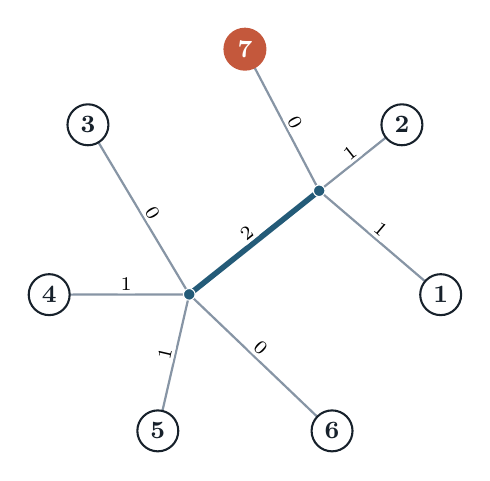
\begin{tikzpicture}[x=1cm,y=1cm]
\coordinate (v1) at (2.48607,-0.56743);
\coordinate (v2) at (1.99367,1.58990);
\coordinate (v3) at (-1.99367,1.58990);
\coordinate (v4) at (-2.48607,-0.56743);
\coordinate (v5) at (-1.10640,-2.29747);
\coordinate (v6) at (1.10640,-2.29747);
\coordinate (v7) at (0.00000,2.55000);
\coordinate (v8) at (0.94310,0.75210);
\coordinate (v9) at (-0.70733,-0.56407);
\draw[internal edge] (v8) -- node[edge label,pos=0.50] {$2$} (v9);
\draw[pendant edge] (v1) -- node[edge label,pos=0.55] {$1$} (v8);
\draw[pendant edge] (v2) -- node[edge label,pos=0.55] {$1$} (v8);
\draw[pendant edge] (v3) -- node[edge label,pos=0.55] {$0$} (v9);
\draw[pendant edge] (v4) -- node[edge label,pos=0.55] {$1$} (v9);
\draw[pendant edge] (v5) -- node[edge label,pos=0.55] {$1$} (v9);
\draw[pendant edge] (v6) -- node[edge label,pos=0.55] {$0$} (v9);
\draw[pendant edge] (v7) -- node[edge label,pos=0.55] {$0$} (v8);
\node[internal vertex] at (v8) {};
\node[internal vertex] at (v9) {};
\node[leaf] at (v1) {1};
\node[leaf] at (v2) {2};
\node[leaf] at (v3) {3};
\node[leaf] at (v4) {4};
\node[leaf] at (v5) {5};
\node[leaf] at (v6) {6};
\node[special leaf] at (v7) {7};
\end{tikzpicture}
\end{minipage}
\par\vspace{1mm}
\begin{minipage}[t][0.285\textheight][t]{0.485\textwidth}
\centering
{\large\bfseries Ray 25}\par
{\scriptsize\color{muted} Coxeter shift $c=(-\frac{21}{2},\,0,\,\frac{21}{2})$}\par
{\scriptsize\color{muted} integral scale $m=2$, diagonal shift $a=-95$, gcd $g=35$}\par\vspace{1mm}
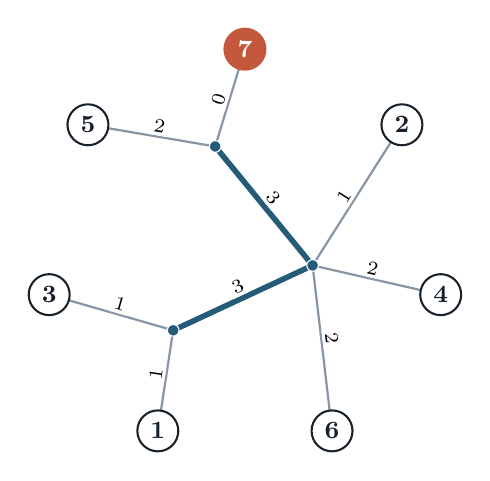
\begin{tikzpicture}[x=1cm,y=1cm]
\coordinate (v1) at (-1.10640,-2.29747);
\coordinate (v2) at (1.99367,1.58990);
\coordinate (v3) at (-2.48607,-0.56743);
\coordinate (v4) at (2.48607,-0.56743);
\coordinate (v5) at (-1.99367,1.58990);
\coordinate (v6) at (1.10640,-2.29747);
\coordinate (v7) at (0.00000,2.55000);
\coordinate (v8) at (-0.91102,-1.02035);
\coordinate (v9) at (-0.37809,1.31458);
\coordinate (v10) at (0.85941,-0.19615);
\draw[internal edge] (v8) -- node[edge label,pos=0.50] {$3$} (v10);
\draw[internal edge] (v9) -- node[edge label,pos=0.50] {$3$} (v10);
\draw[pendant edge] (v1) -- node[edge label,pos=0.55] {$1$} (v8);
\draw[pendant edge] (v2) -- node[edge label,pos=0.55] {$1$} (v10);
\draw[pendant edge] (v3) -- node[edge label,pos=0.55] {$1$} (v8);
\draw[pendant edge] (v4) -- node[edge label,pos=0.55] {$2$} (v10);
\draw[pendant edge] (v5) -- node[edge label,pos=0.55] {$2$} (v9);
\draw[pendant edge] (v6) -- node[edge label,pos=0.55] {$2$} (v10);
\draw[pendant edge] (v7) -- node[edge label,pos=0.55] {$0$} (v9);
\node[internal vertex] at (v8) {};
\node[internal vertex] at (v9) {};
\node[internal vertex] at (v10) {};
\node[leaf] at (v1) {1};
\node[leaf] at (v2) {2};
\node[leaf] at (v3) {3};
\node[leaf] at (v4) {4};
\node[leaf] at (v5) {5};
\node[leaf] at (v6) {6};
\node[special leaf] at (v7) {7};
\end{tikzpicture}
\end{minipage}
\hfill
\begin{minipage}[t][0.285\textheight][t]{0.485\textwidth}
\centering
{\large\bfseries Ray 26}\par
{\scriptsize\color{muted} Coxeter shift $c=(\frac{21}{2},\,-\frac{21}{2},\,0)$}\par
{\scriptsize\color{muted} integral scale $m=2$, diagonal shift $a=-95$, gcd $g=35$}\par\vspace{1mm}
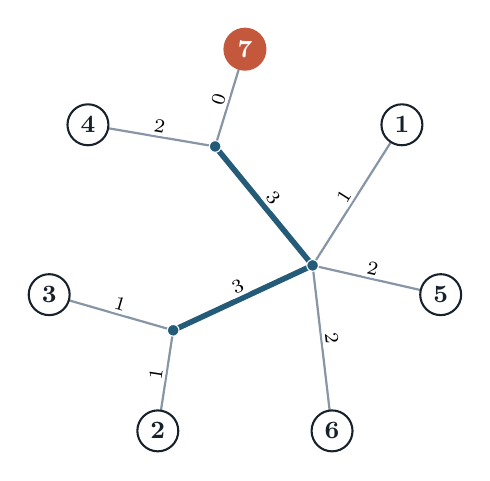
\begin{tikzpicture}[x=1cm,y=1cm]
\coordinate (v1) at (1.99367,1.58990);
\coordinate (v2) at (-1.10640,-2.29747);
\coordinate (v3) at (-2.48607,-0.56743);
\coordinate (v4) at (-1.99367,1.58990);
\coordinate (v5) at (2.48607,-0.56743);
\coordinate (v6) at (1.10640,-2.29747);
\coordinate (v7) at (0.00000,2.55000);
\coordinate (v8) at (-0.91102,-1.02035);
\coordinate (v9) at (-0.37809,1.31458);
\coordinate (v10) at (0.85941,-0.19615);
\draw[internal edge] (v8) -- node[edge label,pos=0.50] {$3$} (v10);
\draw[internal edge] (v9) -- node[edge label,pos=0.50] {$3$} (v10);
\draw[pendant edge] (v1) -- node[edge label,pos=0.55] {$1$} (v10);
\draw[pendant edge] (v2) -- node[edge label,pos=0.55] {$1$} (v8);
\draw[pendant edge] (v3) -- node[edge label,pos=0.55] {$1$} (v8);
\draw[pendant edge] (v4) -- node[edge label,pos=0.55] {$2$} (v9);
\draw[pendant edge] (v5) -- node[edge label,pos=0.55] {$2$} (v10);
\draw[pendant edge] (v6) -- node[edge label,pos=0.55] {$2$} (v10);
\draw[pendant edge] (v7) -- node[edge label,pos=0.55] {$0$} (v9);
\node[internal vertex] at (v8) {};
\node[internal vertex] at (v9) {};
\node[internal vertex] at (v10) {};
\node[leaf] at (v1) {1};
\node[leaf] at (v2) {2};
\node[leaf] at (v3) {3};
\node[leaf] at (v4) {4};
\node[leaf] at (v5) {5};
\node[leaf] at (v6) {6};
\node[special leaf] at (v7) {7};
\end{tikzpicture}
\end{minipage}
\par\vspace{1mm}
\clearpage

\begin{tikzpicture}
\node[rounded corners=2pt,fill=paperblue,inner xsep=5mm,inner ysep=2.2mm,text width=.94\textwidth] {\Large\bfseries Orbit 2 (continued)\hfill\normalsize 12 rays};
\end{tikzpicture}\par\vspace{1mm}
{\small\color{muted} Ray indices: 2, 3, 5, 16, 25, 26, 27, 28, 31, 32, 46, 47}\par\vspace{2mm}
\begin{minipage}[t][0.285\textheight][t]{0.485\textwidth}
\centering
{\large\bfseries Ray 27}\par
{\scriptsize\color{muted} Coxeter shift $c=(0,\,-\frac{7}{2},\,\frac{7}{2})$}\par
{\scriptsize\color{muted} integral scale $m=2$, diagonal shift $a=-120$, gcd $g=105$}\par\vspace{1mm}
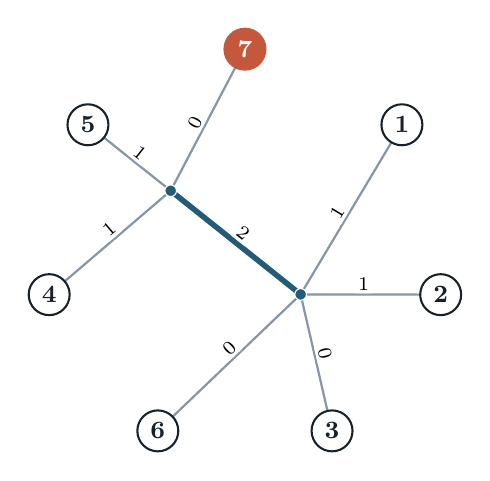
\begin{tikzpicture}[x=1cm,y=1cm]
\coordinate (v1) at (1.99367,1.58990);
\coordinate (v2) at (2.48607,-0.56743);
\coordinate (v3) at (1.10640,-2.29747);
\coordinate (v4) at (-2.48607,-0.56743);
\coordinate (v5) at (-1.99367,1.58990);
\coordinate (v6) at (-1.10640,-2.29747);
\coordinate (v7) at (0.00000,2.55000);
\coordinate (v8) at (-0.94310,0.75210);
\coordinate (v9) at (0.70733,-0.56407);
\draw[internal edge] (v8) -- node[edge label,pos=0.50] {$2$} (v9);
\draw[pendant edge] (v1) -- node[edge label,pos=0.55] {$1$} (v9);
\draw[pendant edge] (v2) -- node[edge label,pos=0.55] {$1$} (v9);
\draw[pendant edge] (v3) -- node[edge label,pos=0.55] {$0$} (v9);
\draw[pendant edge] (v4) -- node[edge label,pos=0.55] {$1$} (v8);
\draw[pendant edge] (v5) -- node[edge label,pos=0.55] {$1$} (v8);
\draw[pendant edge] (v6) -- node[edge label,pos=0.55] {$0$} (v9);
\draw[pendant edge] (v7) -- node[edge label,pos=0.55] {$0$} (v8);
\node[internal vertex] at (v8) {};
\node[internal vertex] at (v9) {};
\node[leaf] at (v1) {1};
\node[leaf] at (v2) {2};
\node[leaf] at (v3) {3};
\node[leaf] at (v4) {4};
\node[leaf] at (v5) {5};
\node[leaf] at (v6) {6};
\node[special leaf] at (v7) {7};
\end{tikzpicture}
\end{minipage}
\hfill
\begin{minipage}[t][0.285\textheight][t]{0.485\textwidth}
\centering
{\large\bfseries Ray 28}\par
{\scriptsize\color{muted} Coxeter shift $c=(0,\,-\frac{21}{2},\,\frac{21}{2})$}\par
{\scriptsize\color{muted} integral scale $m=2$, diagonal shift $a=-95$, gcd $g=35$}\par\vspace{1mm}
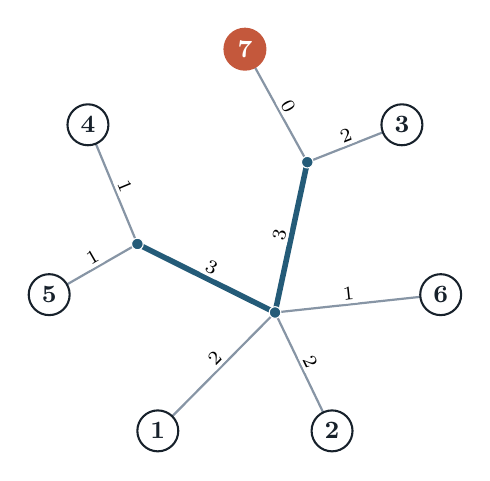
\begin{tikzpicture}[x=1cm,y=1cm]
\coordinate (v1) at (-1.10640,-2.29747);
\coordinate (v2) at (1.10640,-2.29747);
\coordinate (v3) at (1.99367,1.58990);
\coordinate (v4) at (-1.99367,1.58990);
\coordinate (v5) at (-2.48607,-0.56743);
\coordinate (v6) at (2.48607,-0.56743);
\coordinate (v7) at (0.00000,2.55000);
\coordinate (v8) at (0.79205,1.11523);
\coordinate (v9) at (-1.36575,0.07609);
\coordinate (v10) at (0.38247,-0.79421);
\draw[internal edge] (v8) -- node[edge label,pos=0.50] {$3$} (v10);
\draw[internal edge] (v9) -- node[edge label,pos=0.50] {$3$} (v10);
\draw[pendant edge] (v1) -- node[edge label,pos=0.55] {$2$} (v10);
\draw[pendant edge] (v2) -- node[edge label,pos=0.55] {$2$} (v10);
\draw[pendant edge] (v3) -- node[edge label,pos=0.55] {$2$} (v8);
\draw[pendant edge] (v4) -- node[edge label,pos=0.55] {$1$} (v9);
\draw[pendant edge] (v5) -- node[edge label,pos=0.55] {$1$} (v9);
\draw[pendant edge] (v6) -- node[edge label,pos=0.55] {$1$} (v10);
\draw[pendant edge] (v7) -- node[edge label,pos=0.55] {$0$} (v8);
\node[internal vertex] at (v8) {};
\node[internal vertex] at (v9) {};
\node[internal vertex] at (v10) {};
\node[leaf] at (v1) {1};
\node[leaf] at (v2) {2};
\node[leaf] at (v3) {3};
\node[leaf] at (v4) {4};
\node[leaf] at (v5) {5};
\node[leaf] at (v6) {6};
\node[special leaf] at (v7) {7};
\end{tikzpicture}
\end{minipage}
\par\vspace{1mm}
\begin{minipage}[t][0.285\textheight][t]{0.485\textwidth}
\centering
{\large\bfseries Ray 31}\par
{\scriptsize\color{muted} Coxeter shift $c=(-\frac{21}{2},\,\frac{21}{2},\,0)$}\par
{\scriptsize\color{muted} integral scale $m=2$, diagonal shift $a=-95$, gcd $g=35$}\par\vspace{1mm}
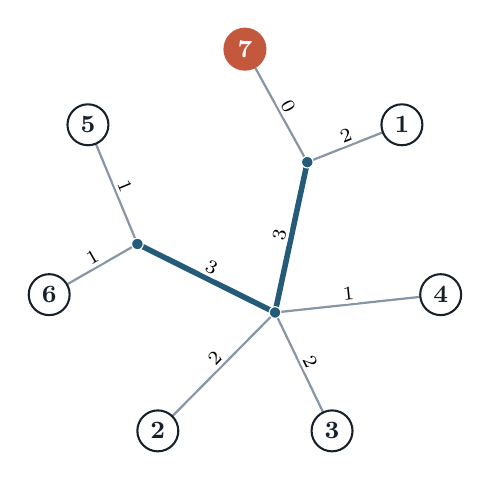
\begin{tikzpicture}[x=1cm,y=1cm]
\coordinate (v1) at (1.99367,1.58990);
\coordinate (v2) at (-1.10640,-2.29747);
\coordinate (v3) at (1.10640,-2.29747);
\coordinate (v4) at (2.48607,-0.56743);
\coordinate (v5) at (-1.99367,1.58990);
\coordinate (v6) at (-2.48607,-0.56743);
\coordinate (v7) at (0.00000,2.55000);
\coordinate (v8) at (0.79205,1.11523);
\coordinate (v9) at (-1.36575,0.07609);
\coordinate (v10) at (0.38247,-0.79421);
\draw[internal edge] (v8) -- node[edge label,pos=0.50] {$3$} (v10);
\draw[internal edge] (v9) -- node[edge label,pos=0.50] {$3$} (v10);
\draw[pendant edge] (v1) -- node[edge label,pos=0.55] {$2$} (v8);
\draw[pendant edge] (v2) -- node[edge label,pos=0.55] {$2$} (v10);
\draw[pendant edge] (v3) -- node[edge label,pos=0.55] {$2$} (v10);
\draw[pendant edge] (v4) -- node[edge label,pos=0.55] {$1$} (v10);
\draw[pendant edge] (v5) -- node[edge label,pos=0.55] {$1$} (v9);
\draw[pendant edge] (v6) -- node[edge label,pos=0.55] {$1$} (v9);
\draw[pendant edge] (v7) -- node[edge label,pos=0.55] {$0$} (v8);
\node[internal vertex] at (v8) {};
\node[internal vertex] at (v9) {};
\node[internal vertex] at (v10) {};
\node[leaf] at (v1) {1};
\node[leaf] at (v2) {2};
\node[leaf] at (v3) {3};
\node[leaf] at (v4) {4};
\node[leaf] at (v5) {5};
\node[leaf] at (v6) {6};
\node[special leaf] at (v7) {7};
\end{tikzpicture}
\end{minipage}
\hfill
\begin{minipage}[t][0.285\textheight][t]{0.485\textwidth}
\centering
{\large\bfseries Ray 32}\par
{\scriptsize\color{muted} Coxeter shift $c=(\frac{21}{2},\,0,\,-\frac{21}{2})$}\par
{\scriptsize\color{muted} integral scale $m=2$, diagonal shift $a=-95$, gcd $g=35$}\par\vspace{1mm}
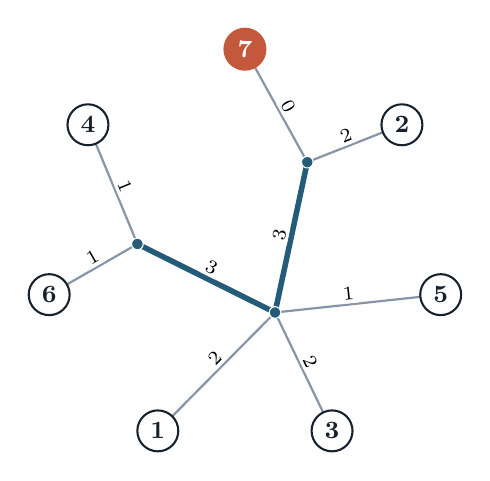
\begin{tikzpicture}[x=1cm,y=1cm]
\coordinate (v1) at (-1.10640,-2.29747);
\coordinate (v2) at (1.99367,1.58990);
\coordinate (v3) at (1.10640,-2.29747);
\coordinate (v4) at (-1.99367,1.58990);
\coordinate (v5) at (2.48607,-0.56743);
\coordinate (v6) at (-2.48607,-0.56743);
\coordinate (v7) at (0.00000,2.55000);
\coordinate (v8) at (0.79205,1.11523);
\coordinate (v9) at (-1.36575,0.07609);
\coordinate (v10) at (0.38247,-0.79421);
\draw[internal edge] (v8) -- node[edge label,pos=0.50] {$3$} (v10);
\draw[internal edge] (v9) -- node[edge label,pos=0.50] {$3$} (v10);
\draw[pendant edge] (v1) -- node[edge label,pos=0.55] {$2$} (v10);
\draw[pendant edge] (v2) -- node[edge label,pos=0.55] {$2$} (v8);
\draw[pendant edge] (v3) -- node[edge label,pos=0.55] {$2$} (v10);
\draw[pendant edge] (v4) -- node[edge label,pos=0.55] {$1$} (v9);
\draw[pendant edge] (v5) -- node[edge label,pos=0.55] {$1$} (v10);
\draw[pendant edge] (v6) -- node[edge label,pos=0.55] {$1$} (v9);
\draw[pendant edge] (v7) -- node[edge label,pos=0.55] {$0$} (v8);
\node[internal vertex] at (v8) {};
\node[internal vertex] at (v9) {};
\node[internal vertex] at (v10) {};
\node[leaf] at (v1) {1};
\node[leaf] at (v2) {2};
\node[leaf] at (v3) {3};
\node[leaf] at (v4) {4};
\node[leaf] at (v5) {5};
\node[leaf] at (v6) {6};
\node[special leaf] at (v7) {7};
\end{tikzpicture}
\end{minipage}
\par\vspace{1mm}
\begin{minipage}[t][0.285\textheight][t]{0.485\textwidth}
\centering
{\large\bfseries Ray 46}\par
{\scriptsize\color{muted} Coxeter shift $c=(-\frac{7}{2},\,0,\,\frac{7}{2})$}\par
{\scriptsize\color{muted} integral scale $m=2$, diagonal shift $a=-120$, gcd $g=105$}\par\vspace{1mm}
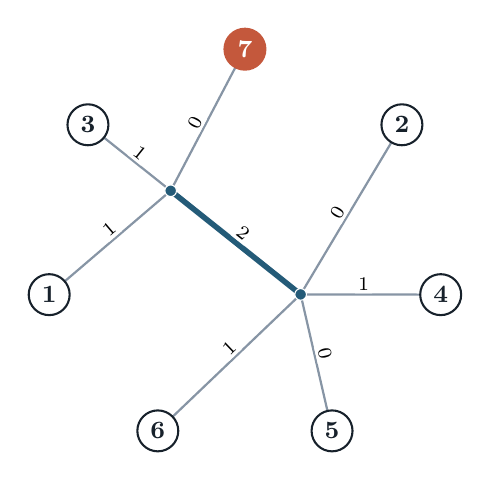
\begin{tikzpicture}[x=1cm,y=1cm]
\coordinate (v1) at (-2.48607,-0.56743);
\coordinate (v2) at (1.99367,1.58990);
\coordinate (v3) at (-1.99367,1.58990);
\coordinate (v4) at (2.48607,-0.56743);
\coordinate (v5) at (1.10640,-2.29747);
\coordinate (v6) at (-1.10640,-2.29747);
\coordinate (v7) at (0.00000,2.55000);
\coordinate (v8) at (-0.94310,0.75210);
\coordinate (v9) at (0.70733,-0.56407);
\draw[internal edge] (v8) -- node[edge label,pos=0.50] {$2$} (v9);
\draw[pendant edge] (v1) -- node[edge label,pos=0.55] {$1$} (v8);
\draw[pendant edge] (v2) -- node[edge label,pos=0.55] {$0$} (v9);
\draw[pendant edge] (v3) -- node[edge label,pos=0.55] {$1$} (v8);
\draw[pendant edge] (v4) -- node[edge label,pos=0.55] {$1$} (v9);
\draw[pendant edge] (v5) -- node[edge label,pos=0.55] {$0$} (v9);
\draw[pendant edge] (v6) -- node[edge label,pos=0.55] {$1$} (v9);
\draw[pendant edge] (v7) -- node[edge label,pos=0.55] {$0$} (v8);
\node[internal vertex] at (v8) {};
\node[internal vertex] at (v9) {};
\node[leaf] at (v1) {1};
\node[leaf] at (v2) {2};
\node[leaf] at (v3) {3};
\node[leaf] at (v4) {4};
\node[leaf] at (v5) {5};
\node[leaf] at (v6) {6};
\node[special leaf] at (v7) {7};
\end{tikzpicture}
\end{minipage}
\hfill
\begin{minipage}[t][0.285\textheight][t]{0.485\textwidth}
\centering
{\large\bfseries Ray 47}\par
{\scriptsize\color{muted} Coxeter shift $c=(\frac{7}{2},\,-\frac{7}{2},\,0)$}\par
{\scriptsize\color{muted} integral scale $m=2$, diagonal shift $a=-120$, gcd $g=105$}\par\vspace{1mm}
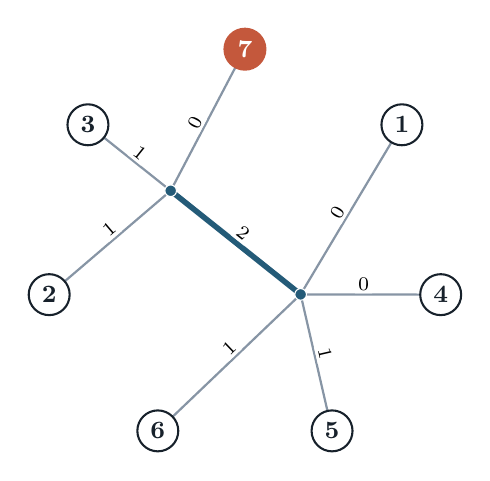
\begin{tikzpicture}[x=1cm,y=1cm]
\coordinate (v1) at (1.99367,1.58990);
\coordinate (v2) at (-2.48607,-0.56743);
\coordinate (v3) at (-1.99367,1.58990);
\coordinate (v4) at (2.48607,-0.56743);
\coordinate (v5) at (1.10640,-2.29747);
\coordinate (v6) at (-1.10640,-2.29747);
\coordinate (v7) at (0.00000,2.55000);
\coordinate (v8) at (-0.94310,0.75210);
\coordinate (v9) at (0.70733,-0.56407);
\draw[internal edge] (v8) -- node[edge label,pos=0.50] {$2$} (v9);
\draw[pendant edge] (v1) -- node[edge label,pos=0.55] {$0$} (v9);
\draw[pendant edge] (v2) -- node[edge label,pos=0.55] {$1$} (v8);
\draw[pendant edge] (v3) -- node[edge label,pos=0.55] {$1$} (v8);
\draw[pendant edge] (v4) -- node[edge label,pos=0.55] {$0$} (v9);
\draw[pendant edge] (v5) -- node[edge label,pos=0.55] {$1$} (v9);
\draw[pendant edge] (v6) -- node[edge label,pos=0.55] {$1$} (v9);
\draw[pendant edge] (v7) -- node[edge label,pos=0.55] {$0$} (v8);
\node[internal vertex] at (v8) {};
\node[internal vertex] at (v9) {};
\node[leaf] at (v1) {1};
\node[leaf] at (v2) {2};
\node[leaf] at (v3) {3};
\node[leaf] at (v4) {4};
\node[leaf] at (v5) {5};
\node[leaf] at (v6) {6};
\node[special leaf] at (v7) {7};
\end{tikzpicture}
\end{minipage}
\par\vspace{1mm}
\clearpage

\begin{tikzpicture}
\node[rounded corners=2pt,fill=paperblue,inner xsep=5mm,inner ysep=2.2mm,text width=.94\textwidth] {\Large\bfseries Orbit 3\hfill\normalsize 6 rays};
\end{tikzpicture}\par\vspace{1mm}
{\small\color{muted} Ray indices: 6, 7, 11, 12, 40, 41}\par\vspace{2mm}
\begin{minipage}[t][0.285\textheight][t]{0.485\textwidth}
\centering
{\large\bfseries Ray 6}\par
{\scriptsize\color{muted} Coxeter shift $c=(-\frac{21}{2},\,-\frac{21}{2},\,21)$}\par
{\scriptsize\color{muted} integral scale $m=2$, diagonal shift $a=-95$, gcd $g=105$}\par\vspace{1mm}
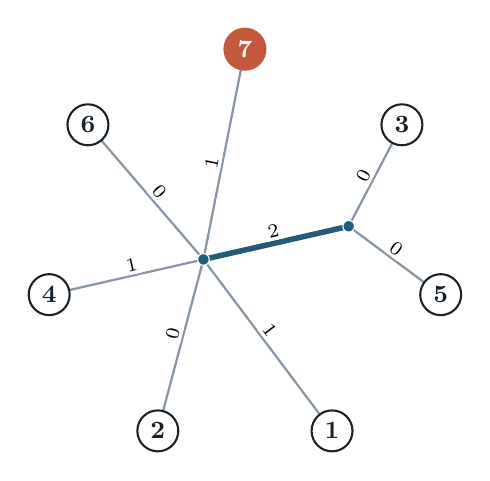
\begin{tikzpicture}[x=1cm,y=1cm]
\coordinate (v1) at (1.10640,-2.29747);
\coordinate (v2) at (-1.10640,-2.29747);
\coordinate (v3) at (1.99367,1.58990);
\coordinate (v4) at (-2.48607,-0.56743);
\coordinate (v5) at (2.48607,-0.56743);
\coordinate (v6) at (-1.99367,1.58990);
\coordinate (v7) at (0.00000,2.55000);
\coordinate (v8) at (1.31757,0.30073);
\coordinate (v9) at (-0.52703,-0.12029);
\draw[internal edge] (v8) -- node[edge label,pos=0.50] {$2$} (v9);
\draw[pendant edge] (v1) -- node[edge label,pos=0.55] {$1$} (v9);
\draw[pendant edge] (v2) -- node[edge label,pos=0.55] {$0$} (v9);
\draw[pendant edge] (v3) -- node[edge label,pos=0.55] {$0$} (v8);
\draw[pendant edge] (v4) -- node[edge label,pos=0.55] {$1$} (v9);
\draw[pendant edge] (v5) -- node[edge label,pos=0.55] {$0$} (v8);
\draw[pendant edge] (v6) -- node[edge label,pos=0.55] {$0$} (v9);
\draw[pendant edge] (v7) -- node[edge label,pos=0.55] {$1$} (v9);
\node[internal vertex] at (v8) {};
\node[internal vertex] at (v9) {};
\node[leaf] at (v1) {1};
\node[leaf] at (v2) {2};
\node[leaf] at (v3) {3};
\node[leaf] at (v4) {4};
\node[leaf] at (v5) {5};
\node[leaf] at (v6) {6};
\node[special leaf] at (v7) {7};
\end{tikzpicture}
\end{minipage}
\hfill
\begin{minipage}[t][0.285\textheight][t]{0.485\textwidth}
\centering
{\large\bfseries Ray 7}\par
{\scriptsize\color{muted} Coxeter shift $c=(\frac{21}{2},\,-21,\,\frac{21}{2})$}\par
{\scriptsize\color{muted} integral scale $m=2$, diagonal shift $a=-95$, gcd $g=105$}\par\vspace{1mm}
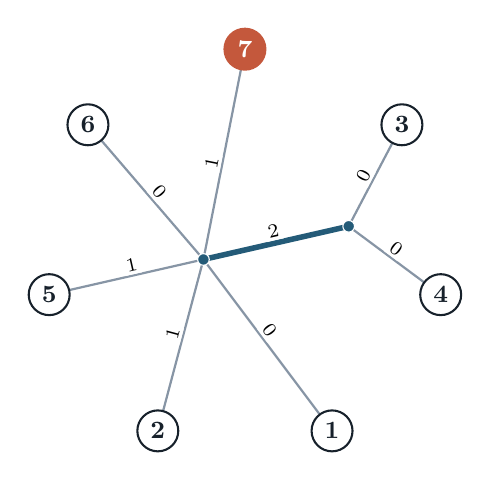
\begin{tikzpicture}[x=1cm,y=1cm]
\coordinate (v1) at (1.10640,-2.29747);
\coordinate (v2) at (-1.10640,-2.29747);
\coordinate (v3) at (1.99367,1.58990);
\coordinate (v4) at (2.48607,-0.56743);
\coordinate (v5) at (-2.48607,-0.56743);
\coordinate (v6) at (-1.99367,1.58990);
\coordinate (v7) at (0.00000,2.55000);
\coordinate (v8) at (1.31757,0.30073);
\coordinate (v9) at (-0.52703,-0.12029);
\draw[internal edge] (v8) -- node[edge label,pos=0.50] {$2$} (v9);
\draw[pendant edge] (v1) -- node[edge label,pos=0.55] {$0$} (v9);
\draw[pendant edge] (v2) -- node[edge label,pos=0.55] {$1$} (v9);
\draw[pendant edge] (v3) -- node[edge label,pos=0.55] {$0$} (v8);
\draw[pendant edge] (v4) -- node[edge label,pos=0.55] {$0$} (v8);
\draw[pendant edge] (v5) -- node[edge label,pos=0.55] {$1$} (v9);
\draw[pendant edge] (v6) -- node[edge label,pos=0.55] {$0$} (v9);
\draw[pendant edge] (v7) -- node[edge label,pos=0.55] {$1$} (v9);
\node[internal vertex] at (v8) {};
\node[internal vertex] at (v9) {};
\node[leaf] at (v1) {1};
\node[leaf] at (v2) {2};
\node[leaf] at (v3) {3};
\node[leaf] at (v4) {4};
\node[leaf] at (v5) {5};
\node[leaf] at (v6) {6};
\node[special leaf] at (v7) {7};
\end{tikzpicture}
\end{minipage}
\par\vspace{1mm}
\begin{minipage}[t][0.285\textheight][t]{0.485\textwidth}
\centering
{\large\bfseries Ray 11}\par
{\scriptsize\color{muted} Coxeter shift $c=(21,\,-\frac{21}{2},\,-\frac{21}{2})$}\par
{\scriptsize\color{muted} integral scale $m=2$, diagonal shift $a=-95$, gcd $g=105$}\par\vspace{1mm}
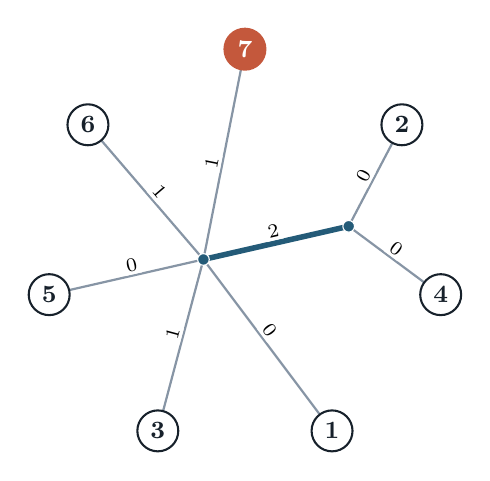
\begin{tikzpicture}[x=1cm,y=1cm]
\coordinate (v1) at (1.10640,-2.29747);
\coordinate (v2) at (1.99367,1.58990);
\coordinate (v3) at (-1.10640,-2.29747);
\coordinate (v4) at (2.48607,-0.56743);
\coordinate (v5) at (-2.48607,-0.56743);
\coordinate (v6) at (-1.99367,1.58990);
\coordinate (v7) at (0.00000,2.55000);
\coordinate (v8) at (1.31757,0.30073);
\coordinate (v9) at (-0.52703,-0.12029);
\draw[internal edge] (v8) -- node[edge label,pos=0.50] {$2$} (v9);
\draw[pendant edge] (v1) -- node[edge label,pos=0.55] {$0$} (v9);
\draw[pendant edge] (v2) -- node[edge label,pos=0.55] {$0$} (v8);
\draw[pendant edge] (v3) -- node[edge label,pos=0.55] {$1$} (v9);
\draw[pendant edge] (v4) -- node[edge label,pos=0.55] {$0$} (v8);
\draw[pendant edge] (v5) -- node[edge label,pos=0.55] {$0$} (v9);
\draw[pendant edge] (v6) -- node[edge label,pos=0.55] {$1$} (v9);
\draw[pendant edge] (v7) -- node[edge label,pos=0.55] {$1$} (v9);
\node[internal vertex] at (v8) {};
\node[internal vertex] at (v9) {};
\node[leaf] at (v1) {1};
\node[leaf] at (v2) {2};
\node[leaf] at (v3) {3};
\node[leaf] at (v4) {4};
\node[leaf] at (v5) {5};
\node[leaf] at (v6) {6};
\node[special leaf] at (v7) {7};
\end{tikzpicture}
\end{minipage}
\hfill
\begin{minipage}[t][0.285\textheight][t]{0.485\textwidth}
\centering
{\large\bfseries Ray 12}\par
{\scriptsize\color{muted} Coxeter shift $c=(-21,\,\frac{21}{2},\,\frac{21}{2})$}\par
{\scriptsize\color{muted} integral scale $m=2$, diagonal shift $a=-95$, gcd $g=105$}\par\vspace{1mm}
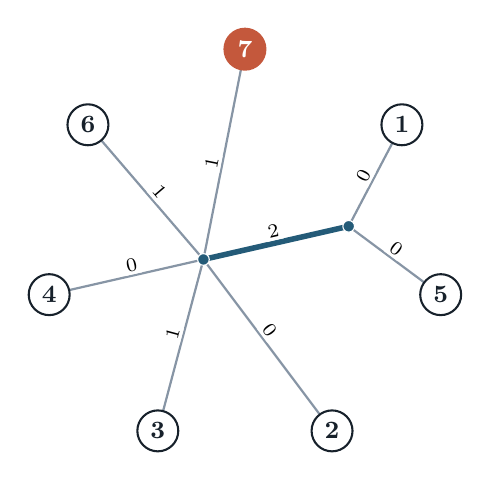
\begin{tikzpicture}[x=1cm,y=1cm]
\coordinate (v1) at (1.99367,1.58990);
\coordinate (v2) at (1.10640,-2.29747);
\coordinate (v3) at (-1.10640,-2.29747);
\coordinate (v4) at (-2.48607,-0.56743);
\coordinate (v5) at (2.48607,-0.56743);
\coordinate (v6) at (-1.99367,1.58990);
\coordinate (v7) at (0.00000,2.55000);
\coordinate (v8) at (1.31757,0.30073);
\coordinate (v9) at (-0.52703,-0.12029);
\draw[internal edge] (v8) -- node[edge label,pos=0.50] {$2$} (v9);
\draw[pendant edge] (v1) -- node[edge label,pos=0.55] {$0$} (v8);
\draw[pendant edge] (v2) -- node[edge label,pos=0.55] {$0$} (v9);
\draw[pendant edge] (v3) -- node[edge label,pos=0.55] {$1$} (v9);
\draw[pendant edge] (v4) -- node[edge label,pos=0.55] {$0$} (v9);
\draw[pendant edge] (v5) -- node[edge label,pos=0.55] {$0$} (v8);
\draw[pendant edge] (v6) -- node[edge label,pos=0.55] {$1$} (v9);
\draw[pendant edge] (v7) -- node[edge label,pos=0.55] {$1$} (v9);
\node[internal vertex] at (v8) {};
\node[internal vertex] at (v9) {};
\node[leaf] at (v1) {1};
\node[leaf] at (v2) {2};
\node[leaf] at (v3) {3};
\node[leaf] at (v4) {4};
\node[leaf] at (v5) {5};
\node[leaf] at (v6) {6};
\node[special leaf] at (v7) {7};
\end{tikzpicture}
\end{minipage}
\par\vspace{1mm}
\begin{minipage}[t][0.285\textheight][t]{0.485\textwidth}
\centering
{\large\bfseries Ray 40}\par
{\scriptsize\color{muted} Coxeter shift $c=(\frac{21}{2},\,\frac{21}{2},\,-21)$}\par
{\scriptsize\color{muted} integral scale $m=2$, diagonal shift $a=-95$, gcd $g=105$}\par\vspace{1mm}
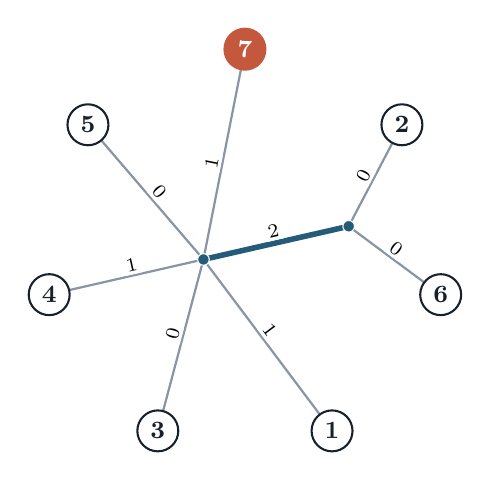
\begin{tikzpicture}[x=1cm,y=1cm]
\coordinate (v1) at (1.10640,-2.29747);
\coordinate (v2) at (1.99367,1.58990);
\coordinate (v3) at (-1.10640,-2.29747);
\coordinate (v4) at (-2.48607,-0.56743);
\coordinate (v5) at (-1.99367,1.58990);
\coordinate (v6) at (2.48607,-0.56743);
\coordinate (v7) at (0.00000,2.55000);
\coordinate (v8) at (1.31757,0.30073);
\coordinate (v9) at (-0.52703,-0.12029);
\draw[internal edge] (v8) -- node[edge label,pos=0.50] {$2$} (v9);
\draw[pendant edge] (v1) -- node[edge label,pos=0.55] {$1$} (v9);
\draw[pendant edge] (v2) -- node[edge label,pos=0.55] {$0$} (v8);
\draw[pendant edge] (v3) -- node[edge label,pos=0.55] {$0$} (v9);
\draw[pendant edge] (v4) -- node[edge label,pos=0.55] {$1$} (v9);
\draw[pendant edge] (v5) -- node[edge label,pos=0.55] {$0$} (v9);
\draw[pendant edge] (v6) -- node[edge label,pos=0.55] {$0$} (v8);
\draw[pendant edge] (v7) -- node[edge label,pos=0.55] {$1$} (v9);
\node[internal vertex] at (v8) {};
\node[internal vertex] at (v9) {};
\node[leaf] at (v1) {1};
\node[leaf] at (v2) {2};
\node[leaf] at (v3) {3};
\node[leaf] at (v4) {4};
\node[leaf] at (v5) {5};
\node[leaf] at (v6) {6};
\node[special leaf] at (v7) {7};
\end{tikzpicture}
\end{minipage}
\hfill
\begin{minipage}[t][0.285\textheight][t]{0.485\textwidth}
\centering
{\large\bfseries Ray 41}\par
{\scriptsize\color{muted} Coxeter shift $c=(-\frac{21}{2},\,21,\,-\frac{21}{2})$}\par
{\scriptsize\color{muted} integral scale $m=2$, diagonal shift $a=-95$, gcd $g=105$}\par\vspace{1mm}
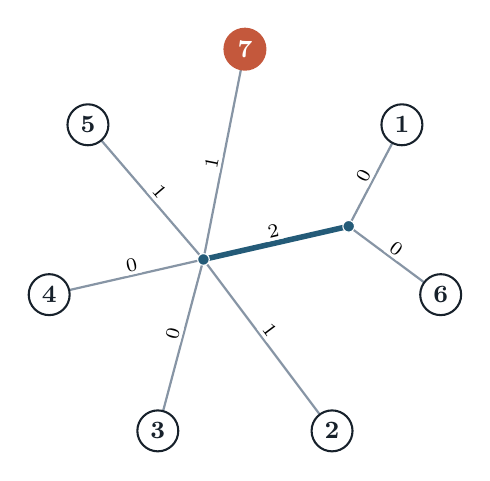
\begin{tikzpicture}[x=1cm,y=1cm]
\coordinate (v1) at (1.99367,1.58990);
\coordinate (v2) at (1.10640,-2.29747);
\coordinate (v3) at (-1.10640,-2.29747);
\coordinate (v4) at (-2.48607,-0.56743);
\coordinate (v5) at (-1.99367,1.58990);
\coordinate (v6) at (2.48607,-0.56743);
\coordinate (v7) at (0.00000,2.55000);
\coordinate (v8) at (1.31757,0.30073);
\coordinate (v9) at (-0.52703,-0.12029);
\draw[internal edge] (v8) -- node[edge label,pos=0.50] {$2$} (v9);
\draw[pendant edge] (v1) -- node[edge label,pos=0.55] {$0$} (v8);
\draw[pendant edge] (v2) -- node[edge label,pos=0.55] {$1$} (v9);
\draw[pendant edge] (v3) -- node[edge label,pos=0.55] {$0$} (v9);
\draw[pendant edge] (v4) -- node[edge label,pos=0.55] {$0$} (v9);
\draw[pendant edge] (v5) -- node[edge label,pos=0.55] {$1$} (v9);
\draw[pendant edge] (v6) -- node[edge label,pos=0.55] {$0$} (v8);
\draw[pendant edge] (v7) -- node[edge label,pos=0.55] {$1$} (v9);
\node[internal vertex] at (v8) {};
\node[internal vertex] at (v9) {};
\node[leaf] at (v1) {1};
\node[leaf] at (v2) {2};
\node[leaf] at (v3) {3};
\node[leaf] at (v4) {4};
\node[leaf] at (v5) {5};
\node[leaf] at (v6) {6};
\node[special leaf] at (v7) {7};
\end{tikzpicture}
\end{minipage}
\par\vspace{1mm}
\clearpage

\begin{tikzpicture}
\node[rounded corners=2pt,fill=paperblue,inner xsep=5mm,inner ysep=2.2mm,text width=.94\textwidth] {\Large\bfseries Orbit 4\hfill\normalsize 6 rays};
\end{tikzpicture}\par\vspace{1mm}
{\small\color{muted} Ray indices: 8, 9, 10, 30, 33, 34}\par\vspace{2mm}
\begin{minipage}[t][0.285\textheight][t]{0.485\textwidth}
\centering
{\large\bfseries Ray 8}\par
{\scriptsize\color{muted} Coxeter shift $c=(0,\,0,\,0)$}\par
{\scriptsize\color{muted} integral scale $m=1$, diagonal shift $a=-2$, gcd $g=7$}\par\vspace{1mm}
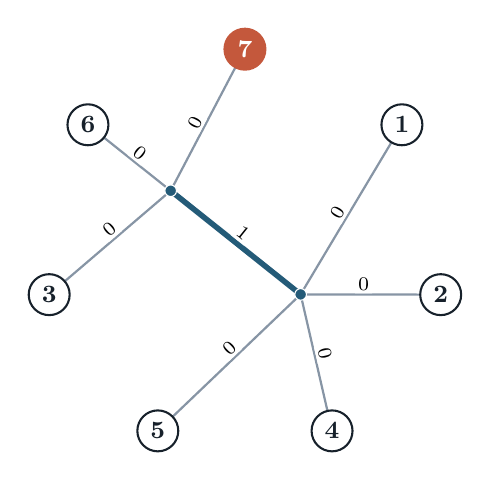
\begin{tikzpicture}[x=1cm,y=1cm]
\coordinate (v1) at (1.99367,1.58990);
\coordinate (v2) at (2.48607,-0.56743);
\coordinate (v3) at (-2.48607,-0.56743);
\coordinate (v4) at (1.10640,-2.29747);
\coordinate (v5) at (-1.10640,-2.29747);
\coordinate (v6) at (-1.99367,1.58990);
\coordinate (v7) at (0.00000,2.55000);
\coordinate (v8) at (-0.94310,0.75210);
\coordinate (v9) at (0.70733,-0.56407);
\draw[internal edge] (v8) -- node[edge label,pos=0.50] {$1$} (v9);
\draw[pendant edge] (v1) -- node[edge label,pos=0.55] {$0$} (v9);
\draw[pendant edge] (v2) -- node[edge label,pos=0.55] {$0$} (v9);
\draw[pendant edge] (v3) -- node[edge label,pos=0.55] {$0$} (v8);
\draw[pendant edge] (v4) -- node[edge label,pos=0.55] {$0$} (v9);
\draw[pendant edge] (v5) -- node[edge label,pos=0.55] {$0$} (v9);
\draw[pendant edge] (v6) -- node[edge label,pos=0.55] {$0$} (v8);
\draw[pendant edge] (v7) -- node[edge label,pos=0.55] {$0$} (v8);
\node[internal vertex] at (v8) {};
\node[internal vertex] at (v9) {};
\node[leaf] at (v1) {1};
\node[leaf] at (v2) {2};
\node[leaf] at (v3) {3};
\node[leaf] at (v4) {4};
\node[leaf] at (v5) {5};
\node[leaf] at (v6) {6};
\node[special leaf] at (v7) {7};
\end{tikzpicture}
\end{minipage}
\hfill
\begin{minipage}[t][0.285\textheight][t]{0.485\textwidth}
\centering
{\large\bfseries Ray 9}\par
{\scriptsize\color{muted} Coxeter shift $c=(0,\,0,\,0)$}\par
{\scriptsize\color{muted} integral scale $m=2$, diagonal shift $a=-20$, gcd $g=21$}\par\vspace{1mm}
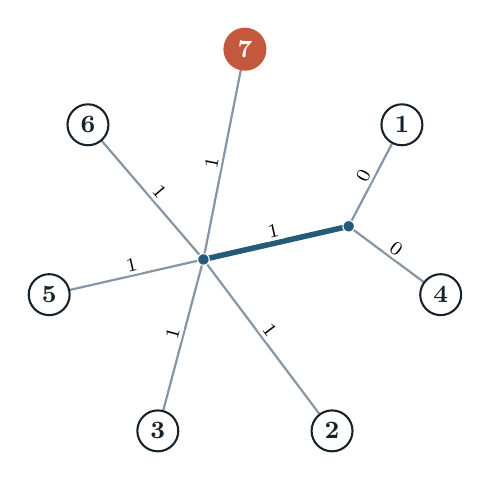
\begin{tikzpicture}[x=1cm,y=1cm]
\coordinate (v1) at (1.99367,1.58990);
\coordinate (v2) at (1.10640,-2.29747);
\coordinate (v3) at (-1.10640,-2.29747);
\coordinate (v4) at (2.48607,-0.56743);
\coordinate (v5) at (-2.48607,-0.56743);
\coordinate (v6) at (-1.99367,1.58990);
\coordinate (v7) at (0.00000,2.55000);
\coordinate (v8) at (1.31757,0.30073);
\coordinate (v9) at (-0.52703,-0.12029);
\draw[internal edge] (v8) -- node[edge label,pos=0.50] {$1$} (v9);
\draw[pendant edge] (v1) -- node[edge label,pos=0.55] {$0$} (v8);
\draw[pendant edge] (v2) -- node[edge label,pos=0.55] {$1$} (v9);
\draw[pendant edge] (v3) -- node[edge label,pos=0.55] {$1$} (v9);
\draw[pendant edge] (v4) -- node[edge label,pos=0.55] {$0$} (v8);
\draw[pendant edge] (v5) -- node[edge label,pos=0.55] {$1$} (v9);
\draw[pendant edge] (v6) -- node[edge label,pos=0.55] {$1$} (v9);
\draw[pendant edge] (v7) -- node[edge label,pos=0.55] {$1$} (v9);
\node[internal vertex] at (v8) {};
\node[internal vertex] at (v9) {};
\node[leaf] at (v1) {1};
\node[leaf] at (v2) {2};
\node[leaf] at (v3) {3};
\node[leaf] at (v4) {4};
\node[leaf] at (v5) {5};
\node[leaf] at (v6) {6};
\node[special leaf] at (v7) {7};
\end{tikzpicture}
\end{minipage}
\par\vspace{1mm}
\begin{minipage}[t][0.285\textheight][t]{0.485\textwidth}
\centering
{\large\bfseries Ray 10}\par
{\scriptsize\color{muted} Coxeter shift $c=(0,\,0,\,0)$}\par
{\scriptsize\color{muted} integral scale $m=2$, diagonal shift $a=-20$, gcd $g=21$}\par\vspace{1mm}
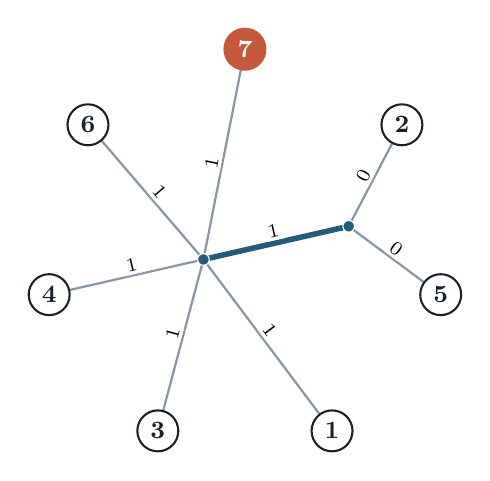
\begin{tikzpicture}[x=1cm,y=1cm]
\coordinate (v1) at (1.10640,-2.29747);
\coordinate (v2) at (1.99367,1.58990);
\coordinate (v3) at (-1.10640,-2.29747);
\coordinate (v4) at (-2.48607,-0.56743);
\coordinate (v5) at (2.48607,-0.56743);
\coordinate (v6) at (-1.99367,1.58990);
\coordinate (v7) at (0.00000,2.55000);
\coordinate (v8) at (1.31757,0.30073);
\coordinate (v9) at (-0.52703,-0.12029);
\draw[internal edge] (v8) -- node[edge label,pos=0.50] {$1$} (v9);
\draw[pendant edge] (v1) -- node[edge label,pos=0.55] {$1$} (v9);
\draw[pendant edge] (v2) -- node[edge label,pos=0.55] {$0$} (v8);
\draw[pendant edge] (v3) -- node[edge label,pos=0.55] {$1$} (v9);
\draw[pendant edge] (v4) -- node[edge label,pos=0.55] {$1$} (v9);
\draw[pendant edge] (v5) -- node[edge label,pos=0.55] {$0$} (v8);
\draw[pendant edge] (v6) -- node[edge label,pos=0.55] {$1$} (v9);
\draw[pendant edge] (v7) -- node[edge label,pos=0.55] {$1$} (v9);
\node[internal vertex] at (v8) {};
\node[internal vertex] at (v9) {};
\node[leaf] at (v1) {1};
\node[leaf] at (v2) {2};
\node[leaf] at (v3) {3};
\node[leaf] at (v4) {4};
\node[leaf] at (v5) {5};
\node[leaf] at (v6) {6};
\node[special leaf] at (v7) {7};
\end{tikzpicture}
\end{minipage}
\hfill
\begin{minipage}[t][0.285\textheight][t]{0.485\textwidth}
\centering
{\large\bfseries Ray 30}\par
{\scriptsize\color{muted} Coxeter shift $c=(0,\,0,\,0)$}\par
{\scriptsize\color{muted} integral scale $m=2$, diagonal shift $a=-20$, gcd $g=21$}\par\vspace{1mm}
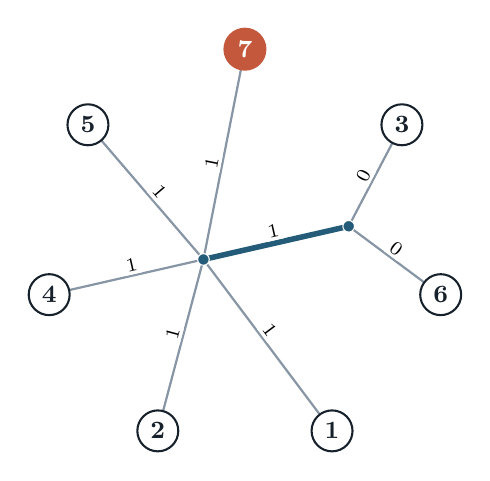
\begin{tikzpicture}[x=1cm,y=1cm]
\coordinate (v1) at (1.10640,-2.29747);
\coordinate (v2) at (-1.10640,-2.29747);
\coordinate (v3) at (1.99367,1.58990);
\coordinate (v4) at (-2.48607,-0.56743);
\coordinate (v5) at (-1.99367,1.58990);
\coordinate (v6) at (2.48607,-0.56743);
\coordinate (v7) at (0.00000,2.55000);
\coordinate (v8) at (1.31757,0.30073);
\coordinate (v9) at (-0.52703,-0.12029);
\draw[internal edge] (v8) -- node[edge label,pos=0.50] {$1$} (v9);
\draw[pendant edge] (v1) -- node[edge label,pos=0.55] {$1$} (v9);
\draw[pendant edge] (v2) -- node[edge label,pos=0.55] {$1$} (v9);
\draw[pendant edge] (v3) -- node[edge label,pos=0.55] {$0$} (v8);
\draw[pendant edge] (v4) -- node[edge label,pos=0.55] {$1$} (v9);
\draw[pendant edge] (v5) -- node[edge label,pos=0.55] {$1$} (v9);
\draw[pendant edge] (v6) -- node[edge label,pos=0.55] {$0$} (v8);
\draw[pendant edge] (v7) -- node[edge label,pos=0.55] {$1$} (v9);
\node[internal vertex] at (v8) {};
\node[internal vertex] at (v9) {};
\node[leaf] at (v1) {1};
\node[leaf] at (v2) {2};
\node[leaf] at (v3) {3};
\node[leaf] at (v4) {4};
\node[leaf] at (v5) {5};
\node[leaf] at (v6) {6};
\node[special leaf] at (v7) {7};
\end{tikzpicture}
\end{minipage}
\par\vspace{1mm}
\begin{minipage}[t][0.285\textheight][t]{0.485\textwidth}
\centering
{\large\bfseries Ray 33}\par
{\scriptsize\color{muted} Coxeter shift $c=(0,\,0,\,0)$}\par
{\scriptsize\color{muted} integral scale $m=1$, diagonal shift $a=-2$, gcd $g=7$}\par\vspace{1mm}
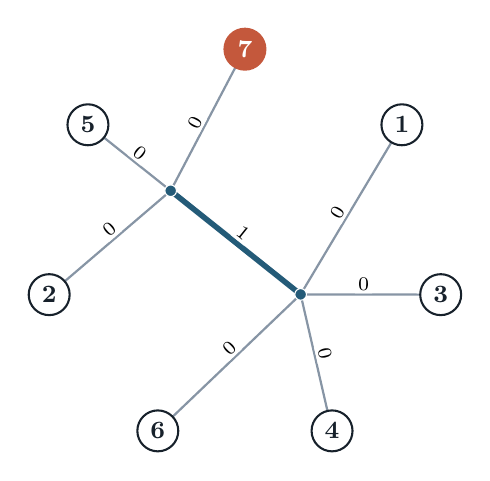
\begin{tikzpicture}[x=1cm,y=1cm]
\coordinate (v1) at (1.99367,1.58990);
\coordinate (v2) at (-2.48607,-0.56743);
\coordinate (v3) at (2.48607,-0.56743);
\coordinate (v4) at (1.10640,-2.29747);
\coordinate (v5) at (-1.99367,1.58990);
\coordinate (v6) at (-1.10640,-2.29747);
\coordinate (v7) at (0.00000,2.55000);
\coordinate (v8) at (-0.94310,0.75210);
\coordinate (v9) at (0.70733,-0.56407);
\draw[internal edge] (v8) -- node[edge label,pos=0.50] {$1$} (v9);
\draw[pendant edge] (v1) -- node[edge label,pos=0.55] {$0$} (v9);
\draw[pendant edge] (v2) -- node[edge label,pos=0.55] {$0$} (v8);
\draw[pendant edge] (v3) -- node[edge label,pos=0.55] {$0$} (v9);
\draw[pendant edge] (v4) -- node[edge label,pos=0.55] {$0$} (v9);
\draw[pendant edge] (v5) -- node[edge label,pos=0.55] {$0$} (v8);
\draw[pendant edge] (v6) -- node[edge label,pos=0.55] {$0$} (v9);
\draw[pendant edge] (v7) -- node[edge label,pos=0.55] {$0$} (v8);
\node[internal vertex] at (v8) {};
\node[internal vertex] at (v9) {};
\node[leaf] at (v1) {1};
\node[leaf] at (v2) {2};
\node[leaf] at (v3) {3};
\node[leaf] at (v4) {4};
\node[leaf] at (v5) {5};
\node[leaf] at (v6) {6};
\node[special leaf] at (v7) {7};
\end{tikzpicture}
\end{minipage}
\hfill
\begin{minipage}[t][0.285\textheight][t]{0.485\textwidth}
\centering
{\large\bfseries Ray 34}\par
{\scriptsize\color{muted} Coxeter shift $c=(0,\,0,\,0)$}\par
{\scriptsize\color{muted} integral scale $m=1$, diagonal shift $a=-2$, gcd $g=7$}\par\vspace{1mm}
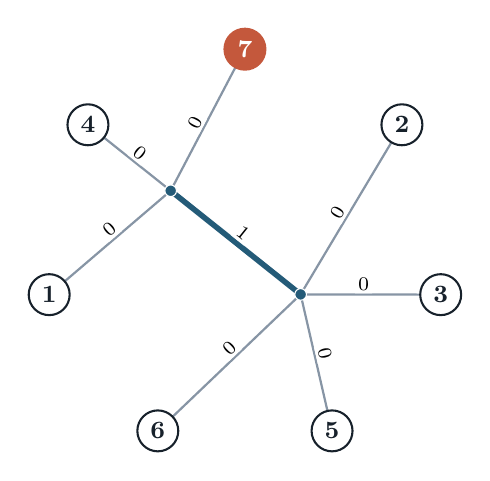
\begin{tikzpicture}[x=1cm,y=1cm]
\coordinate (v1) at (-2.48607,-0.56743);
\coordinate (v2) at (1.99367,1.58990);
\coordinate (v3) at (2.48607,-0.56743);
\coordinate (v4) at (-1.99367,1.58990);
\coordinate (v5) at (1.10640,-2.29747);
\coordinate (v6) at (-1.10640,-2.29747);
\coordinate (v7) at (0.00000,2.55000);
\coordinate (v8) at (-0.94310,0.75210);
\coordinate (v9) at (0.70733,-0.56407);
\draw[internal edge] (v8) -- node[edge label,pos=0.50] {$1$} (v9);
\draw[pendant edge] (v1) -- node[edge label,pos=0.55] {$0$} (v8);
\draw[pendant edge] (v2) -- node[edge label,pos=0.55] {$0$} (v9);
\draw[pendant edge] (v3) -- node[edge label,pos=0.55] {$0$} (v9);
\draw[pendant edge] (v4) -- node[edge label,pos=0.55] {$0$} (v8);
\draw[pendant edge] (v5) -- node[edge label,pos=0.55] {$0$} (v9);
\draw[pendant edge] (v6) -- node[edge label,pos=0.55] {$0$} (v9);
\draw[pendant edge] (v7) -- node[edge label,pos=0.55] {$0$} (v8);
\node[internal vertex] at (v8) {};
\node[internal vertex] at (v9) {};
\node[leaf] at (v1) {1};
\node[leaf] at (v2) {2};
\node[leaf] at (v3) {3};
\node[leaf] at (v4) {4};
\node[leaf] at (v5) {5};
\node[leaf] at (v6) {6};
\node[special leaf] at (v7) {7};
\end{tikzpicture}
\end{minipage}
\par\vspace{1mm}
\clearpage

\begin{tikzpicture}
\node[rounded corners=2pt,fill=paperblue,inner xsep=5mm,inner ysep=2.2mm,text width=.94\textwidth] {\Large\bfseries Orbit 5\hfill\normalsize 6 rays};
\end{tikzpicture}\par\vspace{1mm}
{\small\color{muted} Ray indices: 13, 17, 19, 20, 44, 45}\par\vspace{2mm}
\begin{minipage}[t][0.285\textheight][t]{0.485\textwidth}
\centering
{\large\bfseries Ray 13}\par
{\scriptsize\color{muted} Coxeter shift $c=(0,\,\frac{7}{4},\,-\frac{7}{4})$}\par
{\scriptsize\color{muted} integral scale $m=4$, diagonal shift $a=-220$, gcd $g=35$}\par\vspace{1mm}
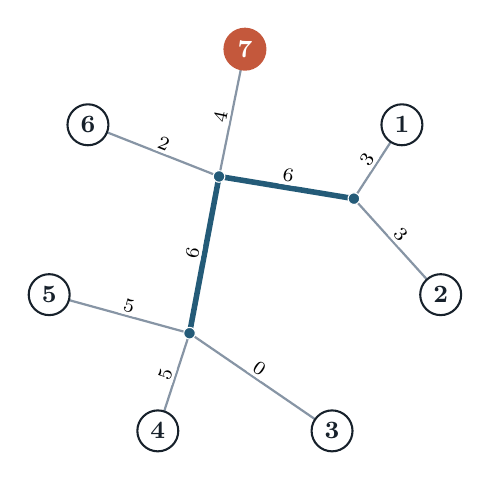
\begin{tikzpicture}[x=1cm,y=1cm]
\coordinate (v1) at (1.99367,1.58990);
\coordinate (v2) at (2.48607,-0.56743);
\coordinate (v3) at (1.10640,-2.29747);
\coordinate (v4) at (-1.10640,-2.29747);
\coordinate (v5) at (-2.48607,-0.56743);
\coordinate (v6) at (-1.99367,1.58990);
\coordinate (v7) at (0.00000,2.55000);
\coordinate (v8) at (1.38379,0.65206);
\coordinate (v9) at (-0.70361,-1.05717);
\coordinate (v10) at (-0.32837,0.93370);
\draw[internal edge] (v8) -- node[edge label,pos=0.50] {$6$} (v10);
\draw[internal edge] (v9) -- node[edge label,pos=0.50] {$6$} (v10);
\draw[pendant edge] (v1) -- node[edge label,pos=0.55] {$3$} (v8);
\draw[pendant edge] (v2) -- node[edge label,pos=0.55] {$3$} (v8);
\draw[pendant edge] (v3) -- node[edge label,pos=0.55] {$0$} (v9);
\draw[pendant edge] (v4) -- node[edge label,pos=0.55] {$5$} (v9);
\draw[pendant edge] (v5) -- node[edge label,pos=0.55] {$5$} (v9);
\draw[pendant edge] (v6) -- node[edge label,pos=0.55] {$2$} (v10);
\draw[pendant edge] (v7) -- node[edge label,pos=0.55] {$4$} (v10);
\node[internal vertex] at (v8) {};
\node[internal vertex] at (v9) {};
\node[internal vertex] at (v10) {};
\node[leaf] at (v1) {1};
\node[leaf] at (v2) {2};
\node[leaf] at (v3) {3};
\node[leaf] at (v4) {4};
\node[leaf] at (v5) {5};
\node[leaf] at (v6) {6};
\node[special leaf] at (v7) {7};
\end{tikzpicture}
\end{minipage}
\hfill
\begin{minipage}[t][0.285\textheight][t]{0.485\textwidth}
\centering
{\large\bfseries Ray 17}\par
{\scriptsize\color{muted} Coxeter shift $c=(0,\,-\frac{7}{4},\,\frac{7}{4})$}\par
{\scriptsize\color{muted} integral scale $m=4$, diagonal shift $a=-220$, gcd $g=35$}\par\vspace{1mm}
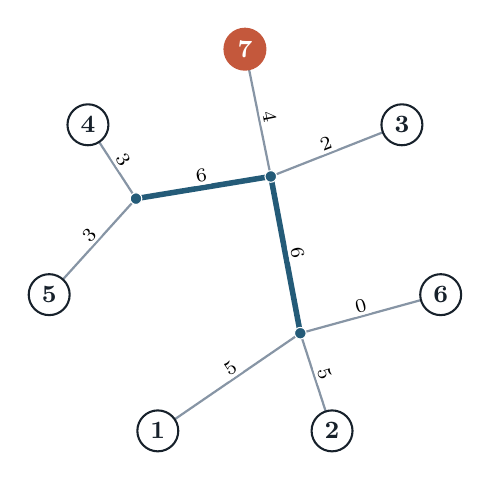
\begin{tikzpicture}[x=1cm,y=1cm]
\coordinate (v1) at (-1.10640,-2.29747);
\coordinate (v2) at (1.10640,-2.29747);
\coordinate (v3) at (1.99367,1.58990);
\coordinate (v4) at (-1.99367,1.58990);
\coordinate (v5) at (-2.48607,-0.56743);
\coordinate (v6) at (2.48607,-0.56743);
\coordinate (v7) at (0.00000,2.55000);
\coordinate (v8) at (-1.38379,0.65206);
\coordinate (v9) at (0.70361,-1.05717);
\coordinate (v10) at (0.32837,0.93370);
\draw[internal edge] (v8) -- node[edge label,pos=0.50] {$6$} (v10);
\draw[internal edge] (v9) -- node[edge label,pos=0.50] {$6$} (v10);
\draw[pendant edge] (v1) -- node[edge label,pos=0.55] {$5$} (v9);
\draw[pendant edge] (v2) -- node[edge label,pos=0.55] {$5$} (v9);
\draw[pendant edge] (v3) -- node[edge label,pos=0.55] {$2$} (v10);
\draw[pendant edge] (v4) -- node[edge label,pos=0.55] {$3$} (v8);
\draw[pendant edge] (v5) -- node[edge label,pos=0.55] {$3$} (v8);
\draw[pendant edge] (v6) -- node[edge label,pos=0.55] {$0$} (v9);
\draw[pendant edge] (v7) -- node[edge label,pos=0.55] {$4$} (v10);
\node[internal vertex] at (v8) {};
\node[internal vertex] at (v9) {};
\node[internal vertex] at (v10) {};
\node[leaf] at (v1) {1};
\node[leaf] at (v2) {2};
\node[leaf] at (v3) {3};
\node[leaf] at (v4) {4};
\node[leaf] at (v5) {5};
\node[leaf] at (v6) {6};
\node[special leaf] at (v7) {7};
\end{tikzpicture}
\end{minipage}
\par\vspace{1mm}
\begin{minipage}[t][0.285\textheight][t]{0.485\textwidth}
\centering
{\large\bfseries Ray 19}\par
{\scriptsize\color{muted} Coxeter shift $c=(-\frac{7}{4},\,\frac{7}{4},\,0)$}\par
{\scriptsize\color{muted} integral scale $m=4$, diagonal shift $a=-220$, gcd $g=35$}\par\vspace{1mm}
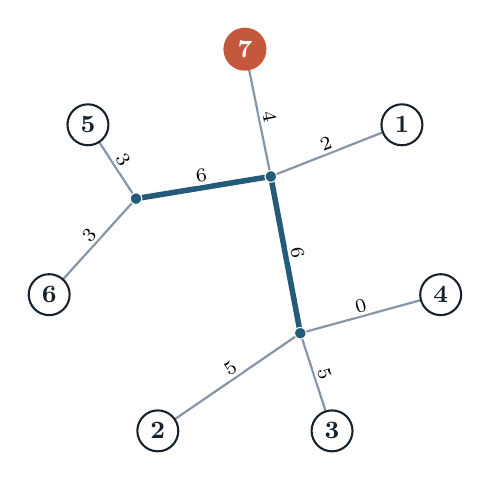
\begin{tikzpicture}[x=1cm,y=1cm]
\coordinate (v1) at (1.99367,1.58990);
\coordinate (v2) at (-1.10640,-2.29747);
\coordinate (v3) at (1.10640,-2.29747);
\coordinate (v4) at (2.48607,-0.56743);
\coordinate (v5) at (-1.99367,1.58990);
\coordinate (v6) at (-2.48607,-0.56743);
\coordinate (v7) at (0.00000,2.55000);
\coordinate (v8) at (-1.38379,0.65206);
\coordinate (v9) at (0.32837,0.93370);
\coordinate (v10) at (0.70361,-1.05717);
\draw[internal edge] (v8) -- node[edge label,pos=0.50] {$6$} (v9);
\draw[internal edge] (v9) -- node[edge label,pos=0.50] {$6$} (v10);
\draw[pendant edge] (v1) -- node[edge label,pos=0.55] {$2$} (v9);
\draw[pendant edge] (v2) -- node[edge label,pos=0.55] {$5$} (v10);
\draw[pendant edge] (v3) -- node[edge label,pos=0.55] {$5$} (v10);
\draw[pendant edge] (v4) -- node[edge label,pos=0.55] {$0$} (v10);
\draw[pendant edge] (v5) -- node[edge label,pos=0.55] {$3$} (v8);
\draw[pendant edge] (v6) -- node[edge label,pos=0.55] {$3$} (v8);
\draw[pendant edge] (v7) -- node[edge label,pos=0.55] {$4$} (v9);
\node[internal vertex] at (v8) {};
\node[internal vertex] at (v9) {};
\node[internal vertex] at (v10) {};
\node[leaf] at (v1) {1};
\node[leaf] at (v2) {2};
\node[leaf] at (v3) {3};
\node[leaf] at (v4) {4};
\node[leaf] at (v5) {5};
\node[leaf] at (v6) {6};
\node[special leaf] at (v7) {7};
\end{tikzpicture}
\end{minipage}
\hfill
\begin{minipage}[t][0.285\textheight][t]{0.485\textwidth}
\centering
{\large\bfseries Ray 20}\par
{\scriptsize\color{muted} Coxeter shift $c=(\frac{7}{4},\,0,\,-\frac{7}{4})$}\par
{\scriptsize\color{muted} integral scale $m=4$, diagonal shift $a=-220$, gcd $g=35$}\par\vspace{1mm}
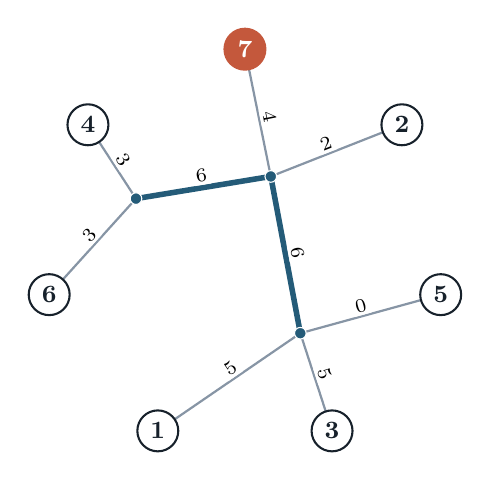
\begin{tikzpicture}[x=1cm,y=1cm]
\coordinate (v1) at (-1.10640,-2.29747);
\coordinate (v2) at (1.99367,1.58990);
\coordinate (v3) at (1.10640,-2.29747);
\coordinate (v4) at (-1.99367,1.58990);
\coordinate (v5) at (2.48607,-0.56743);
\coordinate (v6) at (-2.48607,-0.56743);
\coordinate (v7) at (0.00000,2.55000);
\coordinate (v8) at (-1.38379,0.65206);
\coordinate (v9) at (0.70361,-1.05717);
\coordinate (v10) at (0.32837,0.93370);
\draw[internal edge] (v8) -- node[edge label,pos=0.50] {$6$} (v10);
\draw[internal edge] (v9) -- node[edge label,pos=0.50] {$6$} (v10);
\draw[pendant edge] (v1) -- node[edge label,pos=0.55] {$5$} (v9);
\draw[pendant edge] (v2) -- node[edge label,pos=0.55] {$2$} (v10);
\draw[pendant edge] (v3) -- node[edge label,pos=0.55] {$5$} (v9);
\draw[pendant edge] (v4) -- node[edge label,pos=0.55] {$3$} (v8);
\draw[pendant edge] (v5) -- node[edge label,pos=0.55] {$0$} (v9);
\draw[pendant edge] (v6) -- node[edge label,pos=0.55] {$3$} (v8);
\draw[pendant edge] (v7) -- node[edge label,pos=0.55] {$4$} (v10);
\node[internal vertex] at (v8) {};
\node[internal vertex] at (v9) {};
\node[internal vertex] at (v10) {};
\node[leaf] at (v1) {1};
\node[leaf] at (v2) {2};
\node[leaf] at (v3) {3};
\node[leaf] at (v4) {4};
\node[leaf] at (v5) {5};
\node[leaf] at (v6) {6};
\node[special leaf] at (v7) {7};
\end{tikzpicture}
\end{minipage}
\par\vspace{1mm}
\begin{minipage}[t][0.285\textheight][t]{0.485\textwidth}
\centering
{\large\bfseries Ray 44}\par
{\scriptsize\color{muted} Coxeter shift $c=(-\frac{7}{4},\,0,\,\frac{7}{4})$}\par
{\scriptsize\color{muted} integral scale $m=4$, diagonal shift $a=-220$, gcd $g=35$}\par\vspace{1mm}
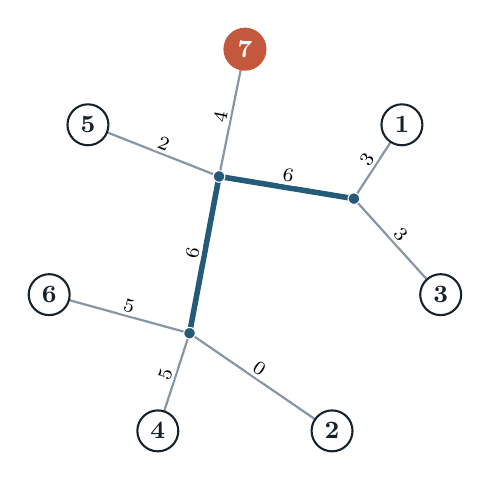
\begin{tikzpicture}[x=1cm,y=1cm]
\coordinate (v1) at (1.99367,1.58990);
\coordinate (v2) at (1.10640,-2.29747);
\coordinate (v3) at (2.48607,-0.56743);
\coordinate (v4) at (-1.10640,-2.29747);
\coordinate (v5) at (-1.99367,1.58990);
\coordinate (v6) at (-2.48607,-0.56743);
\coordinate (v7) at (0.00000,2.55000);
\coordinate (v8) at (1.38379,0.65206);
\coordinate (v9) at (-0.70361,-1.05717);
\coordinate (v10) at (-0.32837,0.93370);
\draw[internal edge] (v8) -- node[edge label,pos=0.50] {$6$} (v10);
\draw[internal edge] (v9) -- node[edge label,pos=0.50] {$6$} (v10);
\draw[pendant edge] (v1) -- node[edge label,pos=0.55] {$3$} (v8);
\draw[pendant edge] (v2) -- node[edge label,pos=0.55] {$0$} (v9);
\draw[pendant edge] (v3) -- node[edge label,pos=0.55] {$3$} (v8);
\draw[pendant edge] (v4) -- node[edge label,pos=0.55] {$5$} (v9);
\draw[pendant edge] (v5) -- node[edge label,pos=0.55] {$2$} (v10);
\draw[pendant edge] (v6) -- node[edge label,pos=0.55] {$5$} (v9);
\draw[pendant edge] (v7) -- node[edge label,pos=0.55] {$4$} (v10);
\node[internal vertex] at (v8) {};
\node[internal vertex] at (v9) {};
\node[internal vertex] at (v10) {};
\node[leaf] at (v1) {1};
\node[leaf] at (v2) {2};
\node[leaf] at (v3) {3};
\node[leaf] at (v4) {4};
\node[leaf] at (v5) {5};
\node[leaf] at (v6) {6};
\node[special leaf] at (v7) {7};
\end{tikzpicture}
\end{minipage}
\hfill
\begin{minipage}[t][0.285\textheight][t]{0.485\textwidth}
\centering
{\large\bfseries Ray 45}\par
{\scriptsize\color{muted} Coxeter shift $c=(\frac{7}{4},\,-\frac{7}{4},\,0)$}\par
{\scriptsize\color{muted} integral scale $m=4$, diagonal shift $a=-220$, gcd $g=35$}\par\vspace{1mm}
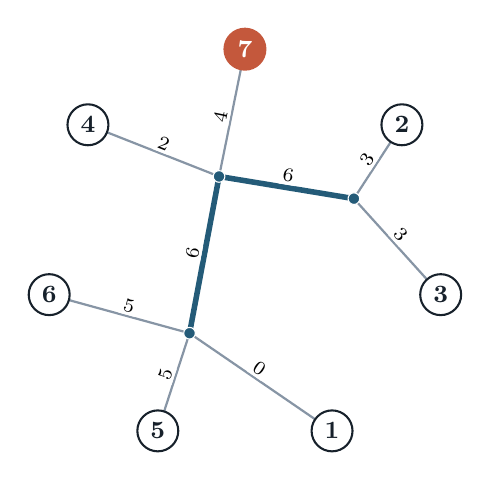
\begin{tikzpicture}[x=1cm,y=1cm]
\coordinate (v1) at (1.10640,-2.29747);
\coordinate (v2) at (1.99367,1.58990);
\coordinate (v3) at (2.48607,-0.56743);
\coordinate (v4) at (-1.99367,1.58990);
\coordinate (v5) at (-1.10640,-2.29747);
\coordinate (v6) at (-2.48607,-0.56743);
\coordinate (v7) at (0.00000,2.55000);
\coordinate (v8) at (1.38379,0.65206);
\coordinate (v9) at (-0.70361,-1.05717);
\coordinate (v10) at (-0.32837,0.93370);
\draw[internal edge] (v8) -- node[edge label,pos=0.50] {$6$} (v10);
\draw[internal edge] (v9) -- node[edge label,pos=0.50] {$6$} (v10);
\draw[pendant edge] (v1) -- node[edge label,pos=0.55] {$0$} (v9);
\draw[pendant edge] (v2) -- node[edge label,pos=0.55] {$3$} (v8);
\draw[pendant edge] (v3) -- node[edge label,pos=0.55] {$3$} (v8);
\draw[pendant edge] (v4) -- node[edge label,pos=0.55] {$2$} (v10);
\draw[pendant edge] (v5) -- node[edge label,pos=0.55] {$5$} (v9);
\draw[pendant edge] (v6) -- node[edge label,pos=0.55] {$5$} (v9);
\draw[pendant edge] (v7) -- node[edge label,pos=0.55] {$4$} (v10);
\node[internal vertex] at (v8) {};
\node[internal vertex] at (v9) {};
\node[internal vertex] at (v10) {};
\node[leaf] at (v1) {1};
\node[leaf] at (v2) {2};
\node[leaf] at (v3) {3};
\node[leaf] at (v4) {4};
\node[leaf] at (v5) {5};
\node[leaf] at (v6) {6};
\node[special leaf] at (v7) {7};
\end{tikzpicture}
\end{minipage}
\par\vspace{1mm}
\clearpage
\begin{tikzpicture}
\node[rounded corners=2pt,fill=paperblue,inner xsep=5mm,inner ysep=2.2mm,text width=.94\textwidth] {\Large\bfseries Orbit 6\hfill\normalsize 3 rays};
\end{tikzpicture}\par\vspace{1mm}
{\small\color{muted} Ray indices: 14, 21, 22}\par\vspace{2mm}
\begin{minipage}[t][0.285\textheight][t]{0.485\textwidth}
\centering
{\large\bfseries Ray 14}\par
{\scriptsize\color{muted} Coxeter shift $c=(0,\,0,\,0)$}\par
{\scriptsize\color{muted} integral scale $m=1$, diagonal shift $a=-10$, gcd $g=21$}\par\vspace{1mm}
\begin{tikzpicture}[x=1cm,y=1cm]
\coordinate (v1) at (1.99367,1.58990);
\coordinate (v2) at (2.48607,-0.56743);
\coordinate (v3) at (-2.48607,-0.56743);
\coordinate (v4) at (1.10640,-2.29747);
\coordinate (v5) at (-1.10640,-2.29747);
\coordinate (v6) at (-1.99367,1.58990);
\coordinate (v7) at (0.00000,2.55000);
\coordinate (v8) at (1.26352,0.52403);
\coordinate (v9) at (-0.22973,-1.34844);
\coordinate (v10) at (-0.68919,0.54961);
\draw[internal edge] (v8) -- node[edge label,pos=0.50] {$1$} (v10);
\draw[internal edge] (v9) -- node[edge label,pos=0.50] {$1$} (v10);
\draw[pendant edge] (v1) -- node[edge label,pos=0.55] {$0$} (v8);
\draw[pendant edge] (v2) -- node[edge label,pos=0.55] {$0$} (v8);
\draw[pendant edge] (v3) -- node[edge label,pos=0.55] {$0$} (v10);
\draw[pendant edge] (v4) -- node[edge label,pos=0.55] {$0$} (v9);
\draw[pendant edge] (v5) -- node[edge label,pos=0.55] {$0$} (v9);
\draw[pendant edge] (v6) -- node[edge label,pos=0.55] {$0$} (v10);
\draw[pendant edge] (v7) -- node[edge label,pos=0.55] {$0$} (v10);
\node[internal vertex] at (v8) {};
\node[internal vertex] at (v9) {};
\node[internal vertex] at (v10) {};
\node[leaf] at (v1) {1};
\node[leaf] at (v2) {2};
\node[leaf] at (v3) {3};
\node[leaf] at (v4) {4};
\node[leaf] at (v5) {5};
\node[leaf] at (v6) {6};
\node[special leaf] at (v7) {7};
\end{tikzpicture}
\end{minipage}
\hfill
\begin{minipage}[t][0.285\textheight][t]{0.485\textwidth}
\centering
{\large\bfseries Ray 21}\par
{\scriptsize\color{muted} Coxeter shift $c=(0,\,0,\,0)$}\par
{\scriptsize\color{muted} integral scale $m=1$, diagonal shift $a=-10$, gcd $g=21$}\par\vspace{1mm}
\begin{tikzpicture}[x=1cm,y=1cm]
\coordinate (v1) at (-2.48607,-0.56743);
\coordinate (v2) at (1.99367,1.58990);
\coordinate (v3) at (2.48607,-0.56743);
\coordinate (v4) at (-1.99367,1.58990);
\coordinate (v5) at (1.10640,-2.29747);
\coordinate (v6) at (-1.10640,-2.29747);
\coordinate (v7) at (0.00000,2.55000);
\coordinate (v8) at (1.26352,0.52403);
\coordinate (v9) at (-0.22973,-1.34844);
\coordinate (v10) at (-0.68919,0.54961);
\draw[internal edge] (v8) -- node[edge label,pos=0.50] {$1$} (v10);
\draw[internal edge] (v9) -- node[edge label,pos=0.50] {$1$} (v10);
\draw[pendant edge] (v1) -- node[edge label,pos=0.55] {$0$} (v10);
\draw[pendant edge] (v2) -- node[edge label,pos=0.55] {$0$} (v8);
\draw[pendant edge] (v3) -- node[edge label,pos=0.55] {$0$} (v8);
\draw[pendant edge] (v4) -- node[edge label,pos=0.55] {$0$} (v10);
\draw[pendant edge] (v5) -- node[edge label,pos=0.55] {$0$} (v9);
\draw[pendant edge] (v6) -- node[edge label,pos=0.55] {$0$} (v9);
\draw[pendant edge] (v7) -- node[edge label,pos=0.55] {$0$} (v10);
\node[internal vertex] at (v8) {};
\node[internal vertex] at (v9) {};
\node[internal vertex] at (v10) {};
\node[leaf] at (v1) {1};
\node[leaf] at (v2) {2};
\node[leaf] at (v3) {3};
\node[leaf] at (v4) {4};
\node[leaf] at (v5) {5};
\node[leaf] at (v6) {6};
\node[special leaf] at (v7) {7};
\end{tikzpicture}
\end{minipage}
\par\vspace{1mm}
\hfill
\begin{minipage}[t][0.285\textheight][t]{0.485\textwidth}
\centering
{\large\bfseries Ray 22}\par
{\scriptsize\color{muted} Coxeter shift $c=(0,\,0,\,0)$}\par
{\scriptsize\color{muted} integral scale $m=1$, diagonal shift $a=-10$, gcd $g=21$}\par\vspace{1mm}
\begin{tikzpicture}[x=1cm,y=1cm]
\coordinate (v1) at (1.99367,1.58990);
\coordinate (v2) at (-2.48607,-0.56743);
\coordinate (v3) at (2.48607,-0.56743);
\coordinate (v4) at (1.10640,-2.29747);
\coordinate (v5) at (-1.99367,1.58990);
\coordinate (v6) at (-1.10640,-2.29747);
\coordinate (v7) at (0.00000,2.55000);
\coordinate (v8) at (1.26352,0.52403);
\coordinate (v9) at (-0.22973,-1.34844);
\coordinate (v10) at (-0.68919,0.54961);
\draw[internal edge] (v8) -- node[edge label,pos=0.50] {$1$} (v10);
\draw[internal edge] (v9) -- node[edge label,pos=0.50] {$1$} (v10);
\draw[pendant edge] (v1) -- node[edge label,pos=0.55] {$0$} (v8);
\draw[pendant edge] (v2) -- node[edge label,pos=0.55] {$0$} (v10);
\draw[pendant edge] (v3) -- node[edge label,pos=0.55] {$0$} (v8);
\draw[pendant edge] (v4) -- node[edge label,pos=0.55] {$0$} (v9);
\draw[pendant edge] (v5) -- node[edge label,pos=0.55] {$0$} (v10);
\draw[pendant edge] (v6) -- node[edge label,pos=0.55] {$0$} (v9);
\draw[pendant edge] (v7) -- node[edge label,pos=0.55] {$0$} (v10);
\node[internal vertex] at (v8) {};
\node[internal vertex] at (v9) {};
\node[internal vertex] at (v10) {};
\node[leaf] at (v1) {1};
\node[leaf] at (v2) {2};
\node[leaf] at (v3) {3};
\node[leaf] at (v4) {4};
\node[leaf] at (v5) {5};
\node[leaf] at (v6) {6};
\node[special leaf] at (v7) {7};
\end{tikzpicture}
\end{minipage}
\hfill\par\vspace{1mm}
\clearpage
\begin{tikzpicture}
\node[rounded corners=2pt,fill=paperblue,inner xsep=5mm,inner ysep=2.2mm,text width=.94\textwidth] {\Large\bfseries Orbit 7\hfill\normalsize 2 rays};
\end{tikzpicture}\par\vspace{1mm}
{\small\color{muted} Ray indices: 15, 29}\par\vspace{2mm}
\begin{minipage}[t][0.285\textheight][t]{0.485\textwidth}
\centering
{\large\bfseries Ray 15}\par
{\scriptsize\color{muted} Coxeter shift $c=(0,\,0,\,0)$}\par
{\scriptsize\color{muted} integral scale $m=2$, diagonal shift $a=-15$, gcd $g=7$}\par\vspace{1mm}
\begin{tikzpicture}[x=1cm,y=1cm]
\coordinate (v1) at (1.99367,1.58990);
\coordinate (v2) at (2.48607,-0.56743);
\coordinate (v3) at (1.10640,-2.29747);
\coordinate (v4) at (-1.10640,-2.29747);
\coordinate (v5) at (-2.48607,-0.56743);
\coordinate (v6) at (-1.99367,1.58990);
\coordinate (v7) at (0.00000,2.55000);
\coordinate (v8) at (1.17603,-0.26842);
\coordinate (v9) at (-0.88202,0.20132);
\draw[internal edge] (v8) -- node[edge label,pos=0.50] {$3$} (v9);
\draw[pendant edge] (v1) -- node[edge label,pos=0.55] {$1$} (v8);
\draw[pendant edge] (v2) -- node[edge label,pos=0.55] {$1$} (v8);
\draw[pendant edge] (v3) -- node[edge label,pos=0.55] {$1$} (v8);
\draw[pendant edge] (v4) -- node[edge label,pos=0.55] {$2$} (v9);
\draw[pendant edge] (v5) -- node[edge label,pos=0.55] {$2$} (v9);
\draw[pendant edge] (v6) -- node[edge label,pos=0.55] {$2$} (v9);
\draw[pendant edge] (v7) -- node[edge label,pos=0.55] {$0$} (v9);
\node[internal vertex] at (v8) {};
\node[internal vertex] at (v9) {};
\node[leaf] at (v1) {1};
\node[leaf] at (v2) {2};
\node[leaf] at (v3) {3};
\node[leaf] at (v4) {4};
\node[leaf] at (v5) {5};
\node[leaf] at (v6) {6};
\node[special leaf] at (v7) {7};
\end{tikzpicture}
\end{minipage}
\hfill
\begin{minipage}[t][0.285\textheight][t]{0.485\textwidth}
\centering
{\large\bfseries Ray 29}\par
{\scriptsize\color{muted} Coxeter shift $c=(0,\,0,\,0)$}\par
{\scriptsize\color{muted} integral scale $m=2$, diagonal shift $a=-15$, gcd $g=7$}\par\vspace{1mm}
\begin{tikzpicture}[x=1cm,y=1cm]
\coordinate (v1) at (1.10640,-2.29747);
\coordinate (v2) at (2.48607,-0.56743);
\coordinate (v3) at (1.99367,1.58990);
\coordinate (v4) at (-1.99367,1.58990);
\coordinate (v5) at (-2.48607,-0.56743);
\coordinate (v6) at (-1.10640,-2.29747);
\coordinate (v7) at (0.00000,2.55000);
\coordinate (v8) at (-1.17603,-0.26842);
\coordinate (v9) at (0.88202,0.20132);
\draw[internal edge] (v8) -- node[edge label,pos=0.50] {$3$} (v9);
\draw[pendant edge] (v1) -- node[edge label,pos=0.55] {$2$} (v9);
\draw[pendant edge] (v2) -- node[edge label,pos=0.55] {$2$} (v9);
\draw[pendant edge] (v3) -- node[edge label,pos=0.55] {$2$} (v9);
\draw[pendant edge] (v4) -- node[edge label,pos=0.55] {$1$} (v8);
\draw[pendant edge] (v5) -- node[edge label,pos=0.55] {$1$} (v8);
\draw[pendant edge] (v6) -- node[edge label,pos=0.55] {$1$} (v8);
\draw[pendant edge] (v7) -- node[edge label,pos=0.55] {$0$} (v9);
\node[internal vertex] at (v8) {};
\node[internal vertex] at (v9) {};
\node[leaf] at (v1) {1};
\node[leaf] at (v2) {2};
\node[leaf] at (v3) {3};
\node[leaf] at (v4) {4};
\node[leaf] at (v5) {5};
\node[leaf] at (v6) {6};
\node[special leaf] at (v7) {7};
\end{tikzpicture}
\end{minipage}
\par\vspace{1mm}
\clearpage
\begin{tikzpicture}
\node[rounded corners=2pt,fill=paperblue,inner xsep=5mm,inner ysep=2.2mm,text width=.94\textwidth] {\Large\bfseries Orbit 8\hfill\normalsize 3 rays};
\end{tikzpicture}\par\vspace{1mm}
{\small\color{muted} Ray indices: 18, 35, 36}\par\vspace{2mm}
\begin{minipage}[t][0.285\textheight][t]{0.485\textwidth}
\centering
{\large\bfseries Ray 18}\par
{\scriptsize\color{muted} Coxeter shift $c=(0,\,0,\,0)$}\par
{\scriptsize\color{muted} integral scale $m=1$, diagonal shift $a=-9$, gcd $g=7$}\par\vspace{1mm}
\begin{tikzpicture}[x=1cm,y=1cm]
\coordinate (v1) at (1.99367,1.58990);
\coordinate (v2) at (2.48607,-0.56743);
\coordinate (v3) at (-1.10640,-2.29747);
\coordinate (v4) at (-2.48607,-0.56743);
\coordinate (v5) at (-1.99367,1.58990);
\coordinate (v6) at (1.10640,-2.29747);
\coordinate (v7) at (0.00000,2.55000);
\coordinate (v8) at (1.39653,-0.12750);
\coordinate (v9) at (0.00000,0.76500);
\coordinate (v10) at (-1.39653,-0.12750);
\draw[internal edge] (v8) -- node[edge label,pos=0.50] {$1$} (v9);
\draw[internal edge] (v9) -- node[edge label,pos=0.50] {$1$} (v10);
\draw[pendant edge] (v1) -- node[edge label,pos=0.55] {$1$} (v8);
\draw[pendant edge] (v2) -- node[edge label,pos=0.55] {$1$} (v8);
\draw[pendant edge] (v3) -- node[edge label,pos=0.55] {$0$} (v10);
\draw[pendant edge] (v4) -- node[edge label,pos=0.55] {$1$} (v10);
\draw[pendant edge] (v5) -- node[edge label,pos=0.55] {$1$} (v10);
\draw[pendant edge] (v6) -- node[edge label,pos=0.55] {$0$} (v8);
\draw[pendant edge] (v7) -- node[edge label,pos=0.55] {$1$} (v9);
\node[internal vertex] at (v8) {};
\node[internal vertex] at (v9) {};
\node[internal vertex] at (v10) {};
\node[leaf] at (v1) {1};
\node[leaf] at (v2) {2};
\node[leaf] at (v3) {3};
\node[leaf] at (v4) {4};
\node[leaf] at (v5) {5};
\node[leaf] at (v6) {6};
\node[special leaf] at (v7) {7};
\end{tikzpicture}
\end{minipage}
\hfill
\begin{minipage}[t][0.285\textheight][t]{0.485\textwidth}
\centering
{\large\bfseries Ray 35}\par
{\scriptsize\color{muted} Coxeter shift $c=(0,\,0,\,0)$}\par
{\scriptsize\color{muted} integral scale $m=1$, diagonal shift $a=-9$, gcd $g=7$}\par\vspace{1mm}
\begin{tikzpicture}[x=1cm,y=1cm]
\coordinate (v1) at (1.99367,1.58990);
\coordinate (v2) at (-1.10640,-2.29747);
\coordinate (v3) at (2.48607,-0.56743);
\coordinate (v4) at (-2.48607,-0.56743);
\coordinate (v5) at (1.10640,-2.29747);
\coordinate (v6) at (-1.99367,1.58990);
\coordinate (v7) at (0.00000,2.55000);
\coordinate (v8) at (1.39653,-0.12750);
\coordinate (v9) at (0.00000,0.76500);
\coordinate (v10) at (-1.39653,-0.12750);
\draw[internal edge] (v8) -- node[edge label,pos=0.50] {$1$} (v9);
\draw[internal edge] (v9) -- node[edge label,pos=0.50] {$1$} (v10);
\draw[pendant edge] (v1) -- node[edge label,pos=0.55] {$1$} (v8);
\draw[pendant edge] (v2) -- node[edge label,pos=0.55] {$0$} (v10);
\draw[pendant edge] (v3) -- node[edge label,pos=0.55] {$1$} (v8);
\draw[pendant edge] (v4) -- node[edge label,pos=0.55] {$1$} (v10);
\draw[pendant edge] (v5) -- node[edge label,pos=0.55] {$0$} (v8);
\draw[pendant edge] (v6) -- node[edge label,pos=0.55] {$1$} (v10);
\draw[pendant edge] (v7) -- node[edge label,pos=0.55] {$1$} (v9);
\node[internal vertex] at (v8) {};
\node[internal vertex] at (v9) {};
\node[internal vertex] at (v10) {};
\node[leaf] at (v1) {1};
\node[leaf] at (v2) {2};
\node[leaf] at (v3) {3};
\node[leaf] at (v4) {4};
\node[leaf] at (v5) {5};
\node[leaf] at (v6) {6};
\node[special leaf] at (v7) {7};
\end{tikzpicture}
\end{minipage}
\par\vspace{1mm}
\hfill
\begin{minipage}[t][0.285\textheight][t]{0.485\textwidth}
\centering
{\large\bfseries Ray 36}\par
{\scriptsize\color{muted} Coxeter shift $c=(0,\,0,\,0)$}\par
{\scriptsize\color{muted} integral scale $m=1$, diagonal shift $a=-9$, gcd $g=7$}\par\vspace{1mm}
\begin{tikzpicture}[x=1cm,y=1cm]
\coordinate (v1) at (1.99367,1.58990);
\coordinate (v2) at (-1.10640,-2.29747);
\coordinate (v3) at (-2.48607,-0.56743);
\coordinate (v4) at (-1.99367,1.58990);
\coordinate (v5) at (2.48607,-0.56743);
\coordinate (v6) at (1.10640,-2.29747);
\coordinate (v7) at (0.00000,2.55000);
\coordinate (v8) at (1.39653,-0.12750);
\coordinate (v9) at (0.00000,0.76500);
\coordinate (v10) at (-1.39653,-0.12750);
\draw[internal edge] (v8) -- node[edge label,pos=0.50] {$1$} (v9);
\draw[internal edge] (v9) -- node[edge label,pos=0.50] {$1$} (v10);
\draw[pendant edge] (v1) -- node[edge label,pos=0.55] {$0$} (v8);
\draw[pendant edge] (v2) -- node[edge label,pos=0.55] {$1$} (v10);
\draw[pendant edge] (v3) -- node[edge label,pos=0.55] {$1$} (v10);
\draw[pendant edge] (v4) -- node[edge label,pos=0.55] {$0$} (v10);
\draw[pendant edge] (v5) -- node[edge label,pos=0.55] {$1$} (v8);
\draw[pendant edge] (v6) -- node[edge label,pos=0.55] {$1$} (v8);
\draw[pendant edge] (v7) -- node[edge label,pos=0.55] {$1$} (v9);
\node[internal vertex] at (v8) {};
\node[internal vertex] at (v9) {};
\node[internal vertex] at (v10) {};
\node[leaf] at (v1) {1};
\node[leaf] at (v2) {2};
\node[leaf] at (v3) {3};
\node[leaf] at (v4) {4};
\node[leaf] at (v5) {5};
\node[leaf] at (v6) {6};
\node[special leaf] at (v7) {7};
\end{tikzpicture}
\end{minipage}
\hfill\par\vspace{1mm}
\clearpage
\begin{tikzpicture}
\node[rounded corners=2pt,fill=paperblue,inner xsep=5mm,inner ysep=2.2mm,text width=.94\textwidth] {\Large\bfseries Orbit 9\hfill\normalsize 1 rays};
\end{tikzpicture}\par\vspace{1mm}
{\small\color{muted} Ray indices: 37}\par\vspace{2mm}
\hfill
\begin{minipage}[t][0.285\textheight][t]{0.485\textwidth}
\centering
{\large\bfseries Ray 37}\par
{\scriptsize\color{muted} Coxeter shift $c=(0,\,0,\,0)$}\par
{\scriptsize\color{muted} integral scale $m=2$, diagonal shift $a=-6$, gcd $g=7$}\par\vspace{1mm}
\begin{tikzpicture}[x=1cm,y=1cm]
\coordinate (v1) at (1.99367,1.58990);
\coordinate (v2) at (1.10640,-2.29747);
\coordinate (v3) at (-2.48607,-0.56743);
\coordinate (v4) at (2.48607,-0.56743);
\coordinate (v5) at (-1.10640,-2.29747);
\coordinate (v6) at (-1.99367,1.58990);
\coordinate (v7) at (0.00000,2.55000);
\coordinate (v8) at (1.49325,0.52971);
\coordinate (v9) at (0.00000,-1.34276);
\coordinate (v10) at (-1.49325,0.52971);
\coordinate (v11) at (0.00000,0.56667);
\draw[internal edge] (v8) -- node[edge label,pos=0.50] {$1$} (v11);
\draw[internal edge] (v9) -- node[edge label,pos=0.50] {$1$} (v11);
\draw[internal edge] (v10) -- node[edge label,pos=0.50] {$1$} (v11);
\draw[pendant edge] (v1) -- node[edge label,pos=0.55] {$0$} (v8);
\draw[pendant edge] (v2) -- node[edge label,pos=0.55] {$0$} (v9);
\draw[pendant edge] (v3) -- node[edge label,pos=0.55] {$0$} (v10);
\draw[pendant edge] (v4) -- node[edge label,pos=0.55] {$0$} (v8);
\draw[pendant edge] (v5) -- node[edge label,pos=0.55] {$0$} (v9);
\draw[pendant edge] (v6) -- node[edge label,pos=0.55] {$0$} (v10);
\draw[pendant edge] (v7) -- node[edge label,pos=0.55] {$1$} (v11);
\node[internal vertex] at (v8) {};
\node[internal vertex] at (v9) {};
\node[internal vertex] at (v10) {};
\node[internal vertex] at (v11) {};
\node[leaf] at (v1) {1};
\node[leaf] at (v2) {2};
\node[leaf] at (v3) {3};
\node[leaf] at (v4) {4};
\node[leaf] at (v5) {5};
\node[leaf] at (v6) {6};
\node[special leaf] at (v7) {7};
\end{tikzpicture}
\end{minipage}
\hfill\par\vspace{1mm}
\end{document}
